\documentclass[12pt,reqno,oneside]{amsart}
\usepackage{import}
%===============================%
%  Packages and basic settings  %
%===============================%
\usepackage[headheight=15pt,rmargin=0.5in,lmargin=0.5in,tmargin=0.75in,bmargin=0.75in]{geometry}
\usepackage{imakeidx}
\usepackage{framed}
\usepackage{amssymb}
\usepackage{amsmath}
\usepackage{mathrsfs}
\usepackage{enumitem}
\usepackage{hyperref}
\usepackage{appendix}
\usepackage[capitalise,noabbrev]{cleveref}
\usepackage{tikz}
\usepackage{tikz-cd}
\usepackage{nomencl}\makenomenclature
\usetikzlibrary{braids,arrows,decorations.markings,calc}

%====================================%
%  Theorems, environments & cleveref  %
%====================================%
\newtheorem{theorem}{Theorem}[section]
\newtheorem{proposition}{Proposition}[section]
\newtheorem{corollary}{Corollary}[section]
\newtheorem{lemma}{Lemma}[section]
\newtheorem{conjecture}{Conjecture}[section]
\newtheorem{remark}{Remark}[section]

\newenvironment{stabular}[2][1]
  {\def\arraystretch{#1}\tabular{#2}}
  {\endtabular}

%==================================%
%  Custom commands & environments  %
%==================================%
\newcommand{\legendre}[2]{\left(\frac{#1}{#2}\right)}
\newcommand{\dlegendre}[2]{\displaystyle{\left(\frac{#1}{#2}\right)}}
\newcommand{\tlegendre}[2]{\textstyle{\left(\frac{#1}{#2}\right)}}
\newcommand{\psum}{\sideset{}{'}\sum}
\newcommand{\asum}{\sideset{}{^{\ast}}\sum}
\newcommand{\tmod}[1]{\ \left(\text{mod }#1\right)}
\newcommand{\xto}[1]{\xrightarrow{#1}}
\newcommand{\xfrom}[1]{\xleftarrow{#1}}
\newcommand{\normal}{\mathrel{\unlhd}}
\newcommand{\mf}{\mathfrak}
\newcommand{\mc}{\mathcal}
\newcommand{\ms}{\mathscr}

\newcommand{\Mat}{\mathrm{Mat}}
\newcommand{\GL}{\mathrm{GL}}
\newcommand{\SL}{\mathrm{SL}}
\newcommand{\PSL}{\mathrm{PSL}}
\renewcommand{\O}{\mathrm{O}}
\newcommand{\SO}{\mathrm{SO}}
\newcommand{\U}{\mathrm{U}}
\newcommand{\Sp}{\mathrm{Sp}}

\newcommand{\N}{\mathbb{N}}
\newcommand{\Z}{\mathbb{Z}}
\newcommand{\Q}{\mathbb{Q}}
\newcommand{\R}{\mathbb{R}}
\newcommand{\C}{\mathbb{C}}
\newcommand{\F}{\mathbb{F}}
\renewcommand{\H}{\mathbb{H}}
\renewcommand{\P}{\mathbb{P}}

\renewcommand{\a}{\alpha}
\renewcommand{\b}{\beta}
\newcommand{\g}{\gamma}
\renewcommand{\d}{\delta}
\newcommand{\z}{\zeta}
\renewcommand{\t}{\theta}
\renewcommand{\i}{\iota}
\renewcommand{\k}{\kappa}
\renewcommand{\l}{\lambda}
\newcommand{\s}{\sigma}
\newcommand{\w}{\omega}

\newcommand{\G}{\Gamma}
\newcommand{\D}{\Delta}
\renewcommand{\L}{\Lambda}
\newcommand{\W}{\Omega}

\newcommand{\e}{\varepsilon}
\newcommand{\vt}{\vartheta}
\newcommand{\vphi}{\varphi}
\newcommand{\emt}{\varnothing}

\newcommand{\x}{\times}
\newcommand{\ox}{\otimes}
\newcommand{\op}{\oplus}
\newcommand{\bigox}{\bigotimes}
\newcommand{\bigop}{\bigoplus}
\newcommand{\del}{\partial}
\newcommand{\<}{\langle}
\renewcommand{\>}{\rangle}
\newcommand{\lf}{\lfloor}
\newcommand{\rf}{\rfloor}
\newcommand{\wtilde}{\widetilde}
\newcommand{\what}{\widehat}
\newcommand{\conj}{\overline}
\newcommand{\cchi}{\conj{\chi}}

\DeclareMathOperator{\id}{\textrm{id}}
\DeclareMathOperator{\sgn}{\mathrm{sgn}}
\DeclareMathOperator{\im}{\mathrm{im}}
\DeclareMathOperator{\rk}{\mathrm{rk}}
\DeclareMathOperator{\tr}{\mathrm{trace}}
\DeclareMathOperator{\nm}{\mathrm{norm}}
\DeclareMathOperator{\ord}{\mathrm{ord}}
\DeclareMathOperator{\Hom}{\mathrm{Hom}}
\DeclareMathOperator{\End}{\mathrm{End}}
\DeclareMathOperator{\Aut}{\mathrm{Aut}}
\DeclareMathOperator{\Tor}{\mathrm{Tor}}
\DeclareMathOperator{\Ann}{\mathrm{Ann}}
\DeclareMathOperator{\Gal}{\mathrm{Gal}}
\DeclareMathOperator{\Trace}{\mathrm{Trace}}
\DeclareMathOperator{\Norm}{\mathrm{Norm}}
\DeclareMathOperator{\Span}{\mathrm{Span}}
\DeclareMathOperator*{\Res}{\mathrm{Res}}
\DeclareMathOperator{\Vol}{\mathrm{Vol}}
\DeclareMathOperator{\Li}{\mathrm{Li}}
\renewcommand{\Re}{\mathrm{Re}}
\renewcommand{\Im}{\mathrm{Im}}

\newcommand{\GH}{\G\backslash\H}
\newcommand{\GG}{\G_{\infty}\backslash\G}

\newenvironment{psmallmatrix}
  {\left(\begin{smallmatrix}}
  {\end{smallmatrix}\right)}

%============%
%  Comments  %
%============%
\newcommand{\todo}[1]{\textcolor{red}{\sf Todo: [#1]}}

%===================%
%  Label reminders  %
%===================%
% [label=(\roman*)]
% [label=(\alph*)]
% [label=(\arabic{enumi})]

%==================%
%  Other settings  %
%==================%
\pgfdeclarelayer{background}
\pgfsetlayers{background,main}
\tikzset{->-/.style={decoration={
  markings,
  mark=at position .5 with {\arrow{>}}},postaction={decorate}}}

%=================%
%  Title & Index  %
%=================%
\title{A quadratic double Dirichlet series II: the number field case}
\author{Henry Twiss}
\date{2024}
\makeindex

\begin{document}

\begin{abstract}
    We construct a quadratic double Dirichlet series $Z(s,w)$ built from single variable quadratic Dirichlet $L$-functions $L(s,\chi)$ over $\Q$. We prove that $Z(s,w)$ admits meromorphic continuation to the $(s,w)$-plane and satisfies a group of functional equations.
\end{abstract}

\maketitle

\section{Preliminaries}
    We present an overview of quadratic Dirichlet $L$-functions over $\Q$. We begin with the Riemann zeta-function. The zeta function $\z(s)$ is defined as the Dirichlet series or Euler product
    \[
        \z(s) = \sum_{m \ge 1}\frac{1}{m^{s}} = \prod_{\text{$p$ prime}}\left(1-\frac{1}{p^{s}}\right)^{-1},
    \]
    for $\Re(s) > 1$. The second equality is an analytic reformulation of the fundamental theorem of arithmetic. The Riemann zeta function also admits meromorphic continuation to $\C$ with a simple pole at $s = 1$ of residue $1$. The functional equation is
    \[
        \pi^{-\frac{s}{2}}\G\left(\frac{s}{2}\right)\z(s) = \pi^{-\frac{1-s}{2}}\G\left(\frac{1-s}{2}\right)\z(1-s).
    \]
    Now we recall characters on $\Z$. They are multiplicative functions $\chi:\Z \to \C$ and form a group under multiplication. The two flavors we will care about are:
    
    \begin{itemize}
        \item Dirichlet characters: multiplicative functions $\chi_{d}:\Z \to \C$ modulo $d \ge 1$ (in that they are $d$-periodic) and such that $\chi_{d}(m) = 0$ if $(m,d) > 1$.
        \item Hilbert characters: The group of characters generated by those that appear in the sign change of reciprocity statements.
    \end{itemize}
    
    The image of a Dirichlet character always lands in the roots of unity. Moreover, $\conj{\chi}$ is the multiplicative inverse to $\chi$ and the Dirichlet characters modulo $d$ form a subgroup under multiplication. This group is always finite and its order is $\vphi(d) = |(\F_{q}[t]/d\F_{q}[t])^{\x}|$. The Dirichlet characters that are of interest to us are those given by the quadratic residue symbol on $\Z$. First let us recall this symbol. For any odd prime $p$ and any $d \in \Z$, we define the quadratic residue symbol $\tlegendre{d}{p}$ by
    \[
        \legendre{d}{p} \equiv d^{\frac{p-1}{2}} \tmod{p} = \begin{cases} 1 & \text{if $x^{2} \equiv d \tmod{p}$ is solvable}, \\ -1 & \text{if $x^{2} \equiv d \tmod{p}$ is not solvable}, \\ 0 & \text{if $d \equiv 0 \tmod{p}$}. \end{cases}
    \]
    This symbol only depends upon $d$ modulo $p$ and is multiplicative in $d$. We can extend the quadratic residue symbol multiplicatively in the denominator. First we define
    \[
        \legendre{d}{-1} = \begin{cases} 1 & \text{if $d \ge 0$}, \\ -1 & \text{if $d < 0$}, \end{cases} \quad \text{and} \quad \legendre{d}{2} = \begin{cases} 1 & \text{if $d \equiv 1,7 \tmod{8}$}, \\ -1 & \text{if $d \equiv 3,5 \tmod{8}$}, \\ 0 & \text{if $d \equiv 0 \tmod{2}$}. \end{cases}
    \]
    If $m = up_{1}^{e_{1}}p_{2}^{e_{2}} \cdots p_{k}^{e_{k}}$ is the prime factorization of $m$ (with $u = \pm1$), then we define
    \[
        \legendre{d}{m} = \legendre{d}{u}\prod_{1 \le i \le k}\legendre{d}{p_{i}}^{e_{i}}.
    \]
    The quadratic residue symbol now makes sense for any $m \in \Z$ and is multiplicative in both $d$ and $m$. The quadratic residue symbol also admits the following reciprocity law:

    \begin{theorem}[Quadratic reciprocity]
        If $d,m \in \Z$ with $(d,m) = 1$, then
        \[
            \legendre{d}{m} = (-1)^{\frac{d^{(2)}-1}{2}\frac{m^{(2)}-1}{2}}\legendre{m}{|d|},
        \]
        where $d^{(2)}$ and $m^{(2)}$ are the parts of $d$ and $m$ relatively prime to $2$ respectively.
    \end{theorem}

    Moreover, we have the additional relations
    \[
        \legendre{-1}{m} = (-1)^{\frac{m^{(2)}-1}{2}} \quad \text{and} \quad \legendre{2}{m} = (-1)^{\frac{m^{2}-1}{8}},
    \]
    and if $m \not\equiv 0 \tmod{2}$, we can write
    \[
        \legendre{-1}{m} = (-1)^{\frac{m-1}{2}} = \begin{cases} 1 & \text{$m \equiv 1 \tmod{4}$}, \\ -1 & \text{$m \equiv 3 \tmod{4}$}, \end{cases} \quad \text{and} \quad \legendre{2}{m} = (-1)^{\frac{m^{2}-1}{8}} = \begin{cases} 1 & \text{$m \equiv 1,7 \tmod{8}$}, \\ -1 & \text{$m \equiv 3,5 \tmod{8}$}. \end{cases}
    \]

    We can now define the quadratic Dirichlet characters. For any square-free $d \in \Z$, define the quadratic Dirichlet character $\chi_{d}$ by the following quadratic residue symbol:
    \[
        \chi_{d}(m) = \begin{cases} \legendre{d}{m} & \text{if $d \equiv 1 \tmod{4}$}, \\ \legendre{4d}{m} & \text{if $d \equiv 2,3 \tmod{4}$}. \end{cases}
    \]
    This quadratic Dirichlet character is attached to the quadratic extension $\Q(\sqrt{d})$. We extend $\chi_{d}$ multiplicatively in the denominator so that $\chi_{d}$ makes sense for any odd $d$. In particular, $\chi_{d}(m) = \pm1$ provided $d$ and $m$ are relatively prime and $\chi_{d}(m) = 0$ if $(m,d) > 1$. Quadratic reciprocity implies that $\chi_{d}$ is a Dirichlet character modulo $|d|$ if $d \equiv 1 \tmod{4}$ and is a Dirichlet character modulo $|4d|$ if $d \equiv 2,3 \tmod{4}$. Indeed, if $d \equiv 1 \tmod{4}$ then $d$ is odd and the sign in quadratic reciprocity is always $1$ so that
    \[
        \chi_{d}(m) = \legendre{m}{|d|},
    \]
    and hence is a quadratic Dirichlet character modulo $|d|$. If $d \equiv 3 \tmod{4}$, then $d$ is again odd and the sign in quadratic reciprocity is $\tlegendre{-1}{m}$ which is a quadratic Dirichlet character modulo $4$ so that
    \[
        \chi_{d}(m) = \legendre{-1}{m}\legendre{m}{|d|},
    \]
    and hence is a Dirichlet character modulo $|4d|$. If $d \equiv 2 \tmod{4}$, first we observe that $\tlegendre{4d}{m} = \tlegendre{8}{m}\tlegendre{\frac{d}{2}}{m}$ where $\tlegendre{8}{m}$ is one of the two primitive quadratic Dirichlet character modulo $8$. Now observe that the sign in quadratic reciprocity for $\tlegendre{\frac{d}{2}}{m}$ is either $1$ or $\tlegendre{-1}{m}$ according to if $\frac{d}{2} \equiv 1,3 \tmod{4}$ respectively. Thus
    \[
        \chi_{d}(m) = \legendre{8}{m}\legendre{m}{|\frac{d}{2}|} \quad \text{or} \quad \chi_{d}(m) = \legendre{-8}{m}\legendre{m}{|\frac{d}{2}|},
    \]
    according to if $\frac{d}{2} \equiv 1,3 \tmod{4}$ respectively, and hence is a quadratic Dirichlet character modulo $|4d|$. We can compactly express all of these cases as follows:
    \[
        \chi_{d}(m) = \begin{cases} \legendre{m}{|d|} & \text{if $d \equiv 1,5 \tmod{8}$}, \\ \legendre{-1}{m}\legendre{m}{|d|} & \text{if $d \equiv 3,7 \tmod{8}$}, \\ \legendre{8}{m}\legendre{m}{|\frac{d}{2}|} & \text{if $d \equiv 2 \tmod{8}$}, \\ \legendre{-8}{m}\legendre{m}{|\frac{d}{2}|} & \text{if $d \equiv 6 \tmod{8}$}. \end{cases}
    \]
    We will also set
    \[
        q(d) = \begin{cases} |d| & \text{if $d \equiv 1 \tmod{4}$}, \\ |4d| & \text{if $d \equiv 2,3 \tmod{4}$}, \end{cases} \quad \text{and} \quad \e_{\chi_{d}} = \frac{\tau(\chi_{d})}{\sqrt{q(d)}} = \begin{cases} 1 & \text{if $d \equiv 1 \tmod{4}$}, \\ 1+i & \text{if $d \equiv 2,3 \tmod{4}$}, \end{cases}
    \]
    where $\tau(\chi_{d})$ is the Gauss sum attached to $\chi_{d}$. We will also require an associated character. For each $\chi_{m}$ (here we are purposely interchanging the roles of $d$ and $m$ to keep consistency with the notation when discussing the quadratic double Dirichlet series later), we define $\wtilde{\chi}_{m}$ by
    \[
        \wtilde{\chi}_{m}(d) = (-1)^{\frac{m^{(2)}-1}{2}\frac{d^{(2)}-1}{2}}\chi_{m}(|d|).
    \]
    By quadratic reciprocity, $\wtilde{\chi}_{m}$ is a quadratic Dirichlet character of the same modulus as $\chi_{m}$ and is multiplicative in $m$. Moreover, we have the identity $\wtilde{\wtilde{\chi}}_{m}(d) = \chi_{m}(|d|)$. Analogously, we set
    \[
        q(m) = \begin{cases} |m| & \text{if $m \equiv 1 \tmod{4}$}, \\ |4m| & \text{if $m \equiv 2,3 \tmod{4}$}, \end{cases} \quad \text{and} \quad \e_{\wtilde{\chi}_{m}} = \frac{\tau(\wtilde{\chi}_{m})}{\sqrt{q(m)}} = \begin{cases} 1 & \text{if $m \equiv 1 \tmod{4}$}, \\ 1+i & \text{if $m \equiv 2,3 \tmod{4}$}, \end{cases}
    \]
    where $\tau(\wtilde{\chi}_{m})$ is the Gauss sum attached to $\wtilde{\chi}_{m}$. We now discuss the Hilbert characters. We will only need four of them: the quadratic Dirichlet characters modulo $8$. They are given as follows:
    \begin{gather*}
        \chi_{1}(m) = \begin{cases} 1 &\text{if $m \not\equiv 0 \tmod{2}$}, \\ 0 &\text{if $m \equiv 0 \tmod{2}$}, \end{cases} \quad \chi_{-1}(m) = \begin{cases} 1 &\text{if $m \equiv 1 \tmod{4}$}, \\ -1 &\text{if $m \equiv 3 \tmod{4}$}, \\ 0 &\text{if $m \equiv 0 \tmod{2}$}, \end{cases} \\ \chi_{2}(m) = \begin{cases} 1 &\text{if $m \equiv 1,7 \tmod{8}$}, \\ -1 &\text{if $m \equiv 3,5 \tmod{8}$}, \\ 0 &\text{if $m \equiv 0 \tmod{2}$}, \end{cases} \quad \chi_{-2}(m) = \begin{cases} 1 &\text{if $m \equiv 1,3 \tmod{8}$}, \\ -1 &\text{if $m \equiv 5,7 \tmod{8}$}, \\ 0 &\text{if $m \equiv 0 \tmod{2}$}. \end{cases}
    \end{gather*}
    In general, we will denote a Hilbert character by $\chi_{a}$ with $a \in \{\pm1,\pm2\}$. The Hilbert characters also satisfy an important orthogonality property:

    \begin{theorem}[Orthogonality of Hilbert characters]
        If $d,m \in \Z$ are odd, then
        \[
            \frac{1}{4}\sum_{a \in \{\pm1,\pm2\}}\chi_{a}(dm) = \begin{cases} 1 & \text{if $d \equiv m \tmod{8}$}, \\ 0 & \text{if $d \not\equiv m \tmod{8}$}. \end{cases}
        \]
    \end{theorem}

    Also, we have the identities
    \[
        \wtilde{\chi}_{a}(m) = \chi_{a}(|m|), \quad \chi_{-1}(m) = \legendre{-1}{m}, \quad \text{and} \quad \chi_{2}(m) = \legendre{2}{m},
    \]
    and the relations
    \[
        \chi_{-2}(m) = \chi_{-1}(m)\chi_{2}(m), \quad \chi_{1}(m) = \chi_{-1}(m)\chi_{-1}(m), \quad \text{and} \quad \chi_{-1}(m) = \chi_{2}(m)\chi_{-2}(m).
    \]
    With the Dirichlet and Hilbert characters introduced, we are ready to discuss the $L$-functions associated to quadratic Dirichlet characters. We define the $L$-function $L(s,\chi_{d})$ attached to $\chi_{d}$ for square-free $d$, by a Dirichlet series or Euler product:
    \[
        L(s,\chi_{d}) = \sum_{m \ge 1}\frac{\chi_{d}(m)}{m^{s}} = \prod_{p \text{ prime}}\left(1-\frac{\chi_{d}(p)}{p^{s}}\right)^{-1}.
    \]
    By definition of the quadratic Dirichlet character, $L(s,\chi_{d}) \ll \z(s)$ for $\Re(s) > 1$ so that $L(s,\chi_{d})$ is locally absolutely uniformly convergent in this region. $L(s,\chi_{d})$ also admits analytic continuation to $\C$. The completed $L$-function $L^{\ast}(s,\chi_{d})$ is defined as
    \[
        L^{\ast}(s,\chi_{d}) = \begin{cases} \pi^{-\frac{s}{2}}\G\left(\frac{s}{2}\right)L(s,\chi_{d}) & \text{if $d > 0$}, \\ \pi^{-\frac{s}{2}}\G\left(\frac{s+1}{2}\right)L(s,\chi_{d}) & \text{if $d < 0$}. \end{cases}
    \]
    We have the functional equation
    \[
        L^{\ast}(s,\chi_{d}) = \e_{\chi_{d}}q(d)^{\frac{1}{2}-s}L^{\ast}(1-s,\chi_{d}),
    \]
    which can be equivalently expressed as
    \[
        L^{\ast}(s,\chi_{d}) = \begin{cases} |d|^{\frac{1}{2}-s}L^{\ast}(1-s,\chi_{d}) & \text{if $d \equiv 1,5 \tmod{8}$}, \\ (1+i)|4d|^{\frac{1}{2}-s}L^{\ast}(1-s,\chi_{d}) & \text{if $d \equiv 2,3,6,7 \tmod{8}$}. \end{cases}
    \]
    Note that the gamma factor depends upon $d$ modulo $8$. This the root cause of an important technical issue later when deriving functional equations for the quadratic double Dirichlet series. Analogously, the Dirichlet $L$-function $L(w,\wtilde{\chi}_{m})$ attached to $\wtilde{\chi}_{m}$ for square-free $m$ is defined by a Dirichlet series or Euler product:
    \[
        L(w,\wtilde{\chi}_{m}) = \sum_{d \ge 1}\frac{\wtilde{\chi}_{m}(d)}{d^{w}} = \prod_{p \text{ prime}}\left(1-\frac{\wtilde{\chi}_{m}(p)}{p^{w}}\right)^{-1}.
    \]
    As for $L(s,\chi_{d})$, $L(w,\wtilde{\chi}_{m}) \ll \z(w)$ for $\Re(w) > 1$ so that $L(w,\wtilde{\chi}_{m})$ is locally absolutely uniformly convergent in this region. Moreover, $L(w,\wtilde{\chi}_{m})$ admits analytic continuation to $\C$ and the completed $L$-function $L^{\ast}(w,\wtilde{\chi}_{m})$ is defined as
    \[
        L^{\ast}(w,\wtilde{\chi}_{m}) = \begin{cases} \pi^{-\frac{w}{2}}\G\left(\frac{w}{2}\right)L(w,\wtilde{\chi}_{m}) & \text{if $m \equiv 1,2,5 \tmod{8}$}, \\ \pi^{-\frac{w}{2}}\G\left(\frac{w+1}{2}\right)L(w,\wtilde{\chi}_{m}) & \text{if $m \equiv 3,6,7 \tmod{8}$}. \end{cases}
    \]
    We have the functional equation
    \[
        L^{\ast}(w,\wtilde{\chi}_{m}) = \e_{\wtilde{\chi}_{m}}q(m)^{\frac{1}{2}-w}L^{\ast}(1-w,\wtilde{\chi}_{m}),
    \]
    which can be equivalently expressed as
    \[
        L^{\ast}(w,\wtilde{\chi}_{m}) = \begin{cases} |m|^{\frac{1}{2}-w}L^{\ast}(1-w,\wtilde{\chi}_{m}) & \text{if $m \equiv 1,5 \tmod{8}$}, \\ (1+i)|4m|^{\frac{1}{2}-w}L^{\ast}(1-w,\wtilde{\chi}_{m}) & \text{if $m \equiv 2,3,6,7 \tmod{8}$}. \end{cases}
    \]
    Analogously, note that the gamma factor depends upon $m$ modulo $8$.

    \begin{remark}
        The definitions for $L(s,\chi_{d})$, $L^{\ast}(s,\chi_{d})$, $L(w,\wtilde{\chi}_{m})$, and $L^{\ast}(w,\wtilde{\chi}_{m})$ work perfectly well even when $d$ and $m$ are not square-free (however the functional equations do not hold). We purposely do not define these $L$-functions, yet, for $d$ and $m$ not necessarily square-free.
    \end{remark}
\section{The Quadratic Double Dirichlet Series}
    We will now define the quadratic double Dirichlet series $Z(s,w)$. For any integer $d \ge 1$, write $d = d_{0}d_{1}^{2}$ where $d_{0}$ is square-free. Equivalently, $d_{0}$ is the square-free part of $d$ and $\frac{d}{d_{0}}$ is a perfect square. The \textbf{quadratic double Dirichlet series} $Z(s,w)$ is defined as
    \[
        Z(s,w) = \sum_{\substack{d \ge 1 \\ (d,2) = 1}}\frac{L^{(2)}(s,\chi_{d_{0}})Q_{d_{0}d_{1}^{2}}(s)}{d^{w}},
    \]
    where $Q_{d_{0}d_{1}^{2}}(s)$ is the \textbf{correction polynomial} defined by
    \[
        Q_{d_{0}d_{1}^{2}}(s) = \sum_{e_{1}e_{2} \mid d_{1}}\mu(e_{1})\chi_{d_{0}}(e_{1})e_{1}^{-s}e_{2}^{1-s} = \sum_{e_{1}e_{2}e_{3} = d_{1}}\mu(e_{1})\chi_{d_{0}}(e_{1})e_{1}^{-s}e_{2}^{1-s},
    \]
    and $\mu$ is the usual M\"obius function. For $\Re(s) > 1$, there is the trivial estimate
    \[
        Q_{d_{0}d_{1}^{2}}(s) \ll \sum_{e_{1}e_{2} \mid d_{1}}1 \ll \s_{0}(d_{1})^{2} \ll_{\e} d^{\e},
    \]
     for any $\e > 0$. As $L(s,\chi_{d_{0}}) \ll 1$ for $\Re(s) > 1$, $Z(s,w)$ is locally absolutely uniformly convergent in the region $\L = \{(s,w) \in \C^{2}:\Re(s) > 1, \Re(w) > 1\}$. It will also be necessary to consider quadratic double Dirichlet series twisted by a pair of Hilbert characters $\chi_{a_{1}}$ and $\chi_{a_{2}}$. The \textbf{quadratic double Dirichlet series} $Z_{a_{1},a_{2}}(s,w)$ twisted by $\chi_{a_{1}}$ and $\chi_{a_{2}}$ is defined as
    \[
        Z_{a_{1},a_{2}}(s,w) = \sum_{\substack{d \ge 1 \\ (d,2) = 1}}\frac{L^{(2)}(s,\chi_{a_{1}d_{0}})\chi_{a_{2}}(d)Q_{d_{0}d_{1}^{2}}(s,\chi_{a_{1}})}{d^{w}},
    \]
    where $Q_{d_{0}d_{1}^{2}}(s,\chi_{a_{1}})$ is the \textbf{correction polynomial} twisted by $\chi_{a_{1}}$ defined by
    \[
        Q_{d_{0}d_{1}^{2}}(s,\chi_{a_{1}}) = \sum_{e_{1}e_{2} \mid d_{1}}\mu(e_{1})\chi_{a_{1}d_{0}}(e_{1})e_{1}^{-s}e_{2}^{1-2s} = \sum_{e_{1}e_{2}e_{3} = d_{1}}\mu(e_{1})\chi_{a_{1}d_{0}}(e_{1})e_{1}^{-s}e_{2}^{1-2s},
    \]
    and $\mu$ is the usual M\"obius function. By definition of the Hilbert characters, we have the analogous bound $Q_{d_{0}d_{1}^{2}}(s,\chi_{a_{1}}) \ll d_{\e}$ so that $Z_{a_{1},a_{2}}(s,w)$ converges locally absolutely uniformly in the same region as $Z(s,w)$ does. In particular, $Z(s,w) = Z_{1,1}(s,w)$. We will also require quadratic double Dirichlet series corresponding to the characters $\wtilde{\chi}_{m}$. Analogously writing $m = m_{0}m_{1}^{2}$, the \textbf{quadratic double Dirichlet series} $\wtilde{Z}(s,w)$ is defined as
    \[
        \wtilde{Z}(w,s) = \sum_{\substack{m \ge 1 \\ (m,2) = 1}}\frac{L^{(2)}(w,\wtilde{\chi}_{m_{0}})Q_{m_{0}m_{1}^{2}}(w)}{m^{s}},
    \]
    where $Q_{d_{0}d_{1}^{2}}(w)$ is the \textbf{correction polynomial} defined by
    \[
        Q_{m_{0}m_{1}^{2}}(w) = \sum_{e_{1}e_{2} \mid m_{1}}\mu(e_{1})\chi_{m_{0}}(e_{1})e_{1}^{-w}e_{2}^{1-w} = \sum_{e_{1}e_{2}e_{3} = m_{1}}\mu(e_{1})\chi_{m_{0}}(e_{1})e_{1}^{-w}e_{2}^{1-w},
    \]
    and $\mu$ is the usual M\"obius function. We have the analogous estimate $Q_{m_{0}m_{1}^{2}}(w) \ll_{\e} m^{\e}$ and as $L(w,\wtilde{\chi}_{m_{0}}) \ll 1$ for $\Re(w) > 1$, $\wtilde{Z}(w,s)$ is locally absolutely uniformly convergent in the same region as $Z(s,w)$. We also need to consider twists by a pair of Hilbert characters $\wtilde{\chi}_{a_{2}}$ and $\wtilde{\chi}_{a_{1}}$. The \textbf{quadratic double Dirichlet series} $\wtilde{Z}_{a_{2},a_{1}}(w,s)$ twisted by $\wtilde{\chi}_{a_{2}}$ and $\wtilde{\chi}_{a_{1}}$ is defined as
    \[
        \wtilde{Z}_{a_{2},a_{1}}(w,s) = \sum_{\substack{m \ge 1 \\ (m,2) = 1}}\frac{L^{(2)}(w,\wtilde{\chi}_{a_{2}m_{0}})\wtilde{\chi}_{a_{1}}(m)Q_{m_{0}m_{1}^{2}}(w,\wtilde{\chi}_{a_{2}})}{m^{s}},
    \]
    where $Q_{m_{0}m_{1}^{2}}(w,\wtilde{\chi}_{a_{2}})$ is the \textbf{correction polynomial} twisted by $\wtilde{\chi}_{a_{2}}$ defined by
    \[
        Q_{m_{0}m_{1}^{2}}(w,\wtilde{\chi}_{a_{2}}) = \sum_{e_{1}e_{2} \mid m_{1}}\mu(e_{1})\wtilde{\chi}_{a_{2}m_{0}}(e_{1})e_{1}^{-w}e_{2}^{1-2w} = \sum_{e_{1}e_{2}e_{3} = m_{1}}\mu(e_{1})\wtilde{\chi}_{a_{2}m_{0}}(e_{1})e_{1}^{-w}e_{2}^{1-2w}.
    \]
    and $\mu$ is the usual M\"obius function. By definition of the Hilbert characters, we have the analogous bound $Q_{m_{0}m_{1}^{2}}(w,\wtilde{\chi}_{a_{2}}) \ll_{\e} m^{\e}$ so that $\wtilde{Z}_{a_{2},a_{1}}(w,s)$ converges locally absolutely uniformly in the same region as $\wtilde{Z}(w,s)$ does. In particular, $\wtilde{Z}(w,s) = \wtilde{Z}_{1,1}(w,s)$.
\section{The Interchange}
    As defined, $Z_{a_{1},a_{2}}(s,w)$ is a sum of $L$-functions, and hence Euler products, in $s$. We will prove an interchange formula for $Z_{a_{1},a_{2}}(s,w)$ which will show that it can be expressed as a sum of $L$-functions in $w$. That is, we want the variables $s$ and $w$ to change places. Precisely:

    \begin{theorem}[Interchange]
        Wherever $Z_{a_{1},a_{2}}(s,w)$ converges locally absolutely uniformly,
        \[
            Z_{a_{1},a_{2}}(s,w) = \sum_{\substack{d \ge 1 \\ (d,2) = 1}}\frac{L^{(2)}(s,\chi_{a_{1}d_{0}})\chi_{a_{2}}(d)Q_{d_{0}d_{1}^{2}}(s,\chi_{a_{1}})}{d^{w}} = \sum_{\substack{m \ge 1 \\ (m,2) = 1}}\frac{L^{(2)}(w,\wtilde{\chi}_{a_{2}m_{0}})\wtilde{\chi}_{a_{1}}(m)Q_{m_{0}m_{1}^{2}}(w,\wtilde{\chi}_{a_{2}})}{m^{s}}.
        \]
        Moreover, the same holds for $\wtilde{Z}_{a_{2},a_{1}}(w,s)$.
    \end{theorem}
    \begin{proof}
        Only the second equality needs to be proved. To do this, first expand the $L$-function $L^{(2)}(s,\chi_{a_{1}d_{0}})$ and polynomial $Q_{d_{0}d_{1}^{2}}(s,\chi_{a_{1}})$ to get
        \begin{align*}
            Z(s,w) &= \sum_{\substack{d \ge 1 \\ (d,2) = 1}}\frac{L^{(2)}(s,\chi_{a_{1}d_{0}})\chi_{a_{2}}(d)Q_{d_{0}d_{1}^{2}}(s,\chi_{a_{1}})}{d^{w}} \\
            &= \sum_{\substack{d \ge 1 \\ (d,2) = 1}}\left(\sum_{\substack{m \ge 1 \\ (m,2) = 1}}\chi_{a_{1}d_{0}}(m)m^{-s}\right)\left(\sum_{e_{1}e_{2} \mid d_{1}}\mu(e_{1})\chi_{a_{1}d_{0}}(e_{1})e_{1}^{-s}e_{2}^{1-2s}\right)\chi_{a_{2}}(d)d^{-w} \\
            &= \sum_{\substack{d,m \ge 1 \\ (dm,2) = 1}}\sum_{e_{1}e_{2} \mid d_{1}}\mu(e_{1})\chi_{a_{2}}(d)\chi_{a_{1}d_{0}}(me_{1})e_{1}^{-s}e_{2}^{1-2s}m^{-s}d^{-w}.
        \end{align*}
        Now $\chi_{a_{1}d_{0}}(me_{1}) = 0$ unless $(d_{0},me_{1}) = 1$. We make this restriction on the sum giving
        \[
            \sum_{\substack{d,m \ge 1 \\ (dm,2) = 1}}\sum_{\substack{e_{1}e_{2} \mid d_{1} \\ (d_{0},me_{1}) = 1}}\mu(e_{1})\chi_{a_{2}}(d)\chi_{a_{1}d_{0}}(me_{1})e_{1}^{-s}e_{2}^{1-2s}m^{-s}d^{-w}.
        \]
        Making the change of variables $me_{1} \to m$ yields
        \[
            \sum_{\substack{d \ge 1 \\ (d,2) = 1}}\sum_{\substack{\substack{m \ge 1 \\ (m,2) = 1} \\ e_{1} \mid m}}\sum_{\substack{e_{1}e_{2} \mid d_{1} \\ (d_{0},m) = 1}}\mu(e_{1})\chi_{a_{2}}(d)\chi_{a_{1}d_{0}}(m)e_{2}^{1-2s}m^{-s}d^{-w}.
        \]
        For fixed $d = d_{0}d_{1}^{2}$ and $e_{2}$, the subsum over $m$ and $e_{1}$ is
        \[
            \sum_{\substack{\substack{m \ge 1 \\ (m,2) = 1} \\ e_{1} \mid m}}\sum_{\substack{e_{1} \mid \frac{d_{1}}{e_{2}} \\ (d_{0},m) = 1}}\mu(e_{1})\chi_{a_{1}d_{0}}(m)m^{-s} = \sum_{\substack{\substack{m \ge 1 \\ (m,2) = 1} \\ (d_{0},m) = 1}}\chi_{a_{1}d_{0}}(m)m^{-s}\left(\sum_{e_{1} \mid \left(\frac{d_{1}}{e_{2}},m\right)}\mu(e_{1})\right).
        \]
        The inner sum over $e_{1}$ of the M\"obius function vanishes unless $\left(\frac{d_{1}}{e_{2}},m\right) = 1$ in which case it is $1$. Therefore the triple sum above becomes
        \[
            \sum_{\substack{d,m \ge 1 \\ (dm,2) = 1}}\sum_{\substack{e_{2} \mid d_{1} \\ \left(\frac{d_{0}d_{1}}{e_{2}},m\right) = 1}}\chi_{a_{2}}(d)\chi_{a_{1}d_{0}}(m)e_{2}^{1-2s}m^{-s}d^{-w}.
        \]
        Making the change of variables $d \to de_{2}^{2}$, the condition $\left(\frac{d_{0}d_{1}}{e_{2}},m\right) = 1$ becomes $(d_{0}d_{1},m) = 1$ which is equivalent to $(d,m) = 1$. Moreover, $\chi_{a_{2}}(de_{2}^{2}) = \chi_{a_{2}}(d)$. Altogether, we obtain
        \[
            \sum_{\substack{\substack{d,m \ge 1 \\ (dm,2) = 1} \\ (d,m) = 1}}\sum_{e_{2}}\chi_{a_{2}}(d)\chi_{a_{1}d_{0}}(m)e_{2}^{1-2s-2w}m^{-s}d^{-w}.
        \]
        Writing $m = m_{0}m_{1}^{2}$ analogously as for $d$, quadratic reciprocity and positivity of $m$ and $d$ together imply $\chi_{d_{0}}(m) = \wtilde{\chi}_{m}(d_{0}) = \wtilde{\chi}_{m_{0}}(d)$ where the last equality holds because $(d,m) = 1$ and both $d_{0}$ and $m_{0}$ differ from $d$ and $m$ respectively by perfect squares. As $\chi_{a_{1}}(m) = \wtilde{\chi}_{a_{1}}(m)$ and $\chi_{a_{2}}(d) = \wtilde{\chi}_{a_{2}}(d)$ (again we use the positivity of $m$ and $d$), the previous fact implies $\chi_{a_{2}}(d)\chi_{a_{1}d_{0}}(m) = \wtilde{\chi}_{a_{1}}(m)\wtilde{\chi}_{a_{2}m_{0}}(d)$ and so our expression becomes
        \[
            \sum_{\substack{\substack{d,m \ge 1 \\ (dm,2) = 1} \\ (d,m) = 1}}\sum_{e_{2}}\wtilde{\chi}_{a_{1}}(m)\wtilde{\chi}_{a_{2}m_{0}}(d)e_{2}^{1-2s-2w}m^{-s}d^{-w}.
        \]
        But now we can reverse the argument with the roles of $d$, $m$, $\chi_{a_{1}}$, and $\chi_{a_{2}}$ interchanged respectively, but with $\wtilde{\chi}_{a_{1}}$ and $\wtilde{\chi}_{a_{2}}$, to obtain
        \[
            Z(s,w) = \sum_{\substack{m \ge 1 \\ (m,2) = 1}}\frac{L^{(2)}(w,\wtilde{\chi}_{a_{2}m_{0}})\wtilde{\chi}_{a_{1}}(m)Q_{m_{0}m_{1}^{2}}(w,\wtilde{\chi}_{a_{2}})}{m^{s}}.
        \]
        Clearly the same holds for $\wtilde{Z}_{a_{2},a_{1}}(w,s)$.
    \end{proof}

    Note that the interchange is not completely symmetric because of the characters $\wtilde{\chi}_{a_{2}m_{0}}$, $\wtilde{\chi}_{a_{1}}$, and $\wtilde{\chi}_{a_{2}}$ in the second expression for $Z_{a_{1},a_{2}}(s,w)$. This is due to the fact that reciprocity is not perfect. In even more general settings the correction polynomials in $w$ need not be equal to those in $s$.

    \begin{remark}\label{rem:symmetry_of_Double_Dirichlet_series}
        When $a_{1} = a_{2} = 1$, the interchange implies
        \[
            Z(s,w) = \wtilde{Z}(w,s).
        \]
        More generally, the interchange implies the following relations for twisted quadratic double Dirichlet series:
        \[
            Z_{a_{1},a_{2}}(s,w) = \wtilde{Z}_{a_{2},a_{1}}(w,s),
        \]
        for $a_{1},a_{2} \in \{\pm1,\pm2\}$.
    \end{remark}
\section{Weighting Terms}
    We will now study the coefficients of $Z_{a_{1},a_{2}}(s,w)$ expanded in $s$ and $w$. Expanding $L^{(2)}(s,\chi_{a_{1}d_{0}})Q_{d_{0}d_{1}^{2}}(s,\chi_{a_{1}})$ in the numerator of $Z_{a_{1},a_{2}}(s,w)$, we can write
    \[
        Z_{a_{1},a_{2}}(s,w) = \sum_{\substack{d \ge 1 \\ (d,2) = 1}}\frac{L^{(2)}(s,\chi_{a_{1}d_{0}})\chi_{a_{2}}(d)Q_{d_{0}d_{1}^{2}}(s,\chi_{a_{1}})}{d^{w}} = \sum_{\substack{d,m \ge 1 \\ (dm,2) = 1}}\frac{\chi_{a_{1}d_{0}}(\what{m})\chi_{a_{2}}(d)H(m,d)}{m^{s}d^{w}},
    \]
    where $\what{m}$ is the part of $m$ relatively prime to $d_{0}$ and the \textbf{weighting coefficient} $H(m,d)$ is given by
    \[
        H(m,d) = \sum_{\substack{e_{1}e_{2}^{2}e_{3} = m \\ e_{1}e_{2} \mid d_{1} \\ (d_{0},e_{1}e_{3}) = 1}}\mu(e_{1})e_{2}.
    \]
    To see this, the coefficient of $m^{-s}d^{-w}$ in the definition of $Z_{a_{1},a_{2}}(s,w)$ is
    \begin{align*}
        \chi_{a_{2}}(d)\sum_{\substack{e_{1}e_{2}^{2}e_{3} = m \\ e_{1}e_{2} \mid d_{1}}}\mu(e_{1})\chi_{a_{1}d_{0}}(e_{1}e_{3})e_{2} &= \chi_{a_{2}}(d)\sum_{\substack{e_{1}e_{2}^{2}e_{3} = m \\ e_{1}e_{2} \mid d_{1} \\ (d_{0},e_{1}e_{3}) = 1}}\mu(e_{1})\chi_{a_{1}d_{0}}(e_{1}e_{3})e_{2} \\
        &= \chi_{a_{1}d_{0}}(\what{m})\chi_{a_{2}}(d)\sum_{\substack{e_{1}e_{2}^{2}e_{3} = m \\ e_{1}e_{2} \mid d_{1} \\ (d_{0},e_{1}e_{3}) = 1}}\mu(e_{1})e_{2} \\
        &= \chi_{a_{1}d_{0}}(\what{m})\chi_{a_{2}}(d)H(m,d),
    \end{align*}
    where the first equality holds because $\chi_{d_{0}}(e_{1}e_{3}) = 0$ unless $(d_{0},e_{1}e_{3}) = 1$ and the second equality holds because if $(d_{0},e_{1}e_{3}) = 1$, $\what{m}$ differs from $e_{1}e_{3}$ by a perfect square (the divisors of which belong to $(d_{0},e_{2})$) and so $\chi_{d_{0}}(e_{1}e_{3}) = \chi_{d_{0}}(\what{m})$. For completeness, we extend the definition of $H(m,d)$ to all $d,m \ge 1$. In particular, $H(m,d)$ makes sense when $m$ or $d$ may be even.
    
    \begin{remark}\label{rem:weighting_coefficient_remark}
        Also, $H(m,d) = 0$ unless $m = e_{1}e_{2}^{2}e_{3}$ with $(d_{0},e_{1}e_{3}) = 1$ and $e_{1}e_{2}^{2} \mid d_{1}$.
    \end{remark}

    We will define $L(s,\chi_{a_{1}d})$ to be the Dirichlet series given by
    \[
        L(s,\chi_{a_{1}d}) = L(s,\chi_{a_{1}d_{0}})Q_{d_{0}d_{1}^{2}}(s,\chi_{a_{1}}) = \sum_{m \ge 1}\frac{\chi_{a_{1}d_{0}}(\what{m})H(m,d)}{m^{s}}.
    \]
    Clearly $L(s,\chi_{a_{1}d})$ is locally absolutely uniformly convergent for $\Re(s) > 1$. In particular, $L(s,\chi_{d})$ now makes sense for $d$ not necessarily square-free and this definition agrees with the former when $d$ is square-free. Moreover, we have the representation
    \[
        Z_{a_{1},a_{2}}(s,w) = \sum_{\substack{d \ge 1 \\ (d,2) = 1}}\frac{\chi_{a_{2}}(d)L^{(2)}(s,\chi_{a_{1}d})}{d^{w}}.
    \]
    If we perform the same procedure but with the interchange, we get
    \[
        \wtilde{Z}_{a_{2},a_{1}}(w,s) = \sum_{\substack{m \ge 1 \\ (m,2) = 1}}\frac{L^{(2)}(w,\wtilde{\chi}_{a_{2}m_{0}})\wtilde{\chi}_{a_{1}}(m)Q_{m_{0}m_{1}^{2}}(w,\wtilde{\chi}_{a_{2}})}{m^{s}} = \sum_{\substack{d,m \ge 1 \\ (dm,2) = 1}}\frac{\wtilde{\chi}_{a_{2}m_{0}}(\what{d})\wtilde{\chi}_{a_{1}}(m)H(d,m)}{m^{s}d^{w}},
    \]
    where $\what{d}$ is the part of $d$ relatively prime to $m_{0}$. Analogously, we define $L(w,\wtilde{\chi}_{a_{2}m})$ to be the Dirichlet series given by
    \[
        L(w,\wtilde{\chi}_{a_{2}m}) = L(w,\wtilde{\chi}_{a_{2}m_{0}})Q_{m_{0}m_{1}^{2}}(w,\wtilde{\chi}_{a_{2}}) = \sum_{d \ge 1}\frac{\wtilde{\chi}_{a_{2}m_{0}}(\what{d})H(d,m)}{d^{w}}.
    \]
    Again, $L(w,\wtilde{\chi}_{a_{2}m})$ is locally absolutely uniformly convergent for $\Re(w) > 1$. We also have
    \[
        \wtilde{Z}_{a_{2},a_{1}}(w,s) = \sum_{\substack{m \ge 1 \\ (m,2) = 1}}\frac{\wtilde{\chi}_{a_{1}}(m)L^{(2)}(w,\wtilde{\chi}_{a_{2}m})}{m^{s}}.
    \]
    We now investigate the structure of the weighting coefficients $H(m,d)$. Their structure controls the majority of the information about both the quadratic double Dirichlet series and the correction polynomials. We first show that the weighting coefficients possess a multiplicativity property:

    \begin{proposition}\label{prop:multiplicativity_of_weighting_coefficients}
        We have $H(m,1) = H(1,d) = 1$ and
        \[
            H(m,d) = \prod_{\substack{p^{\a} \mid\mid m \\ p^{\b} \mid\mid d}}H(p^{\a},p^{\b}).
        \]
    \end{proposition}
    \begin{proof}
        From the definition of the weighting coefficients, $H(m,1) = H(1,d) = 1$. We will prove multiplicativity in $m$ and then in $d$. Letting $m = m'p^{\a}$, we must show
        \[
            H(m,d) = H(m',d)H(p^{\a},d).
        \]
        To accomplish this, for $e_{1}e_{2}^{2}e_{3} = m$, let $e_{1} = c_{1}d_{1}$, $e_{2} = c_{2}d_{2}$, and $e_{3} = c_{3}d_{3}$ with $c_{1},c_{2},c_{3} \mid m'$ and $d_{1},d_{2},d_{3} \mid p^{\a}$. Because $(m',p^{\a}) = 1$, as $e_{1}e_{2}^{2}e_{3}$ runs over decompositions of $m$, $c_{1}c_{2}^{2}c_{3}$ and $d_{1}d_{2}^{2}d_{3}$ run over decompositions of $m'$ and $p^{\a}$ respectively. Moreover, as $e_{1}e_{2}$ runs over the divisors of $d_{1}$ so does $c_{1}d_{1}c_{2}d_{2}$. These facts combined with multiplicativity of the M\"obius function gives
        \begin{align*}
            H(m,d) &= \sum_{\substack{e_{1}e_{2}^{2}e_{3} = m \\ e_{1}e_{2} \mid d_{1} \\ (d_{0},e_{1}e_{3}) = 1}}\mu(e_{1})e_{2} \\
            &= \sum_{\substack{c_{1}c_{2}^{2}c_{3} = m' \\ d_{1}d_{2}^{2}d_{3} = p^{\b} \\ c_{1}d_{1}c_{2}d_{2} \mid d_{1} \\ (d_{0},c_{1}d_{1}c_{3}d_{3}) = 1}}\mu(c_{1})(d_{1})|c_{2}|d_{2} \\
            &= \left(\sum_{\substack{c_{1}c_{2}^{2}c_{3} = m' \\ c_{1}c_{2} \mid d_{1} \\ (d_{0},c_{1}c_{3}) = 1}}\mu(c_{1})|c_{2}|\right)\left(\sum_{\substack{d_{1}d_{2}^{2}d_{3} = p^{\a} \\ d_{1}d_{2} \mid d_{1} \\ (d_{0},d_{1}d_{3}) = 1}}\mu(d_{1})d_{2}\right) \\
            &= H(m',d)H(p^{\a},d),
        \end{align*}
        as desired. Now we prove multiplicativity in $d$. Since we have already proven multiplicativity in $m$, we may assume $m = p^{\a}$. Letting $d = d'p^{\b}$, we must show
        \[
            H(p^{\a},d) = H(p^{\a},p^{\b}).
        \]
        As $e_{1}e_{2}^{2}e_{3} = p^{\a}$, the $e_{i}$ are powers of $p$ for $1 \le i \le 3$. It follows that $e_{1}e_{2} \mid d_{1}$ is equivalent to $e_{1}e_{2} \mid p^{\b}$. Moreover, $(d_{0},e_{1}e_{2}) = 1$ is equivalent to $(1,e_{1}e_{2}) = 1$ or $(p,e_{1}e_{2}) = 1$ depending on of $\b$ is even or odd. These facts imply the desired identity.
    \end{proof}

    The correction polynomials $Q_{d_{0}d_{1}^{2}}(s,\chi_{a_{1}})$ are tightly connected to the weighting coefficients $H(m,d)$. In particular, $Q_{d_{0}d_{1}^{2}}(s,\chi_{a_{1}})$ is a Dirichlet polynomial whose coefficients are essentially given by the weighting coefficients. We first prove this relationship when $d$ is an odd prime power:

    \begin{lemma}\label{lem:prime_correction_odd}
        For any prime $p$ and $\a \ge 1$, we have
        \[
            Q_{p^{2\a+1}}(s) = \sum_{k \le 2\a}\frac{H(p^{k},p^{2\a+1})}{p^{ks}}.
        \]
        Moreover, the same holds for $Q_{p^{2\a+1}}(w)$.
    \end{lemma}
    \begin{proof}
        Expanding the correction polynomial in $p^{-s}$ yields
        \[
            Q_{p^{2\a+1}}(s) = \sum_{e_{1}e_{2} \mid p^{\a}}\mu(e_{1})\chi_{p}(e_{1})e_{1}^{-s}e_{2}^{1-2s} = \sum_{k \le 2\a}\frac{H'(p^{k},p^{2\a+1})}{p^{ks}}.
        \]
        where
        \[
            H'(p^{k},p^{2\a+1}) = \sum_{e_{1}e_{2}^{2} = p^{k}}\mu(e_{1})\chi_{p}(e_{1})e_{2}.
        \]
        The proof will be finished if we can show $H'(p^{k},p^{2\a+1}) = H(p^{k},p^{2\a+1})$. To see this, first observe $\mu(e_{1})\chi_{p}(e_{1}) = 0$ unless $e_{1} = 1$ in which case it is $1$. So $H'(p^{k},p^{2\a+1}) = 0$ if $k$ is odd and $p^{\frac{k}{2}}$ if $k$ is even. Compactly stated,
        \[
            H'(p^{k},p^{2\a+1}) = \begin{cases} p^{\frac{k}{2}} & \text{if $k$ is even}, \\ 0 & \text{if $k$ is odd}. \end{cases}
        \]
        On the other hand, $k \le \a$ so that
        \[
            H(p^{k},p^{2\a+1}) = \sum_{\substack{e_{1}e_{2}^{2}e_{3} = p^{k} \\ e_{1}e_{2} \mid p^{\a} \\ (p,e_{1}e_{3}) = 1}}\mu(e_{1})e_{2} = \sum_{\substack{e_{1}e_{2}^{2} \mid p^{k} \\ (p,e_{1}e_{3}) = 1}}\mu(e_{1})e_{2} = \sum_{e_{2}^{2} = p^{k}}e_{2} =  \begin{cases} p^{\frac{k}{2}} & \text{if $k$ is even}, \\ 0 & \text{if $k$ is odd}. \end{cases}
        \]
        This finishes the proof. Clearly the same holds for $Q_{p^{2\a+1}}(w)$.
    \end{proof}

    There is an analogous statement when $d$ is an even prime power up to a square-free factor and relatively prime factor:
    
    \begin{lemma}\label{lem:prime_correction_even}
        For any square-free integer $d_{0} \ge 1$, $a_{1} \in \{\pm1,\pm2\}$, prime $p$ not dividing $d_{0}$, and $\b \ge 1$, we have
        \[
            Q_{d_{0}p^{2\b}}(s,\chi_{a_{1}}) = (1-\chi_{a_{1}d_{0}}(p)p^{-s})\sum_{k \le 2\b}\frac{\chi_{a_{1}d_{0}}(p^{k})H(p^{k},p^{2\b})}{p^{ks}}.
        \]
        Moreover, the same holds for $Q_{m_{0}p^{2\b}}(w,\wtilde{\chi}_{a_{2}})$.
    \end{lemma}
    \begin{proof}
        Expand the correction polynomial in $p^{-s}$ to get
        \[
            Q_{d_{0}p^{2\b}}(s,\chi_{a_{1}}) = \sum_{e_{1}e_{2} \mid p^{\a}}\mu(e_{1})\chi_{a_{1}d_{0}}(e_{1})e_{1}^{-s}e_{2}^{1-2s} = \sum_{k \le 2\b}\frac{H'(p^{k},p^{2\b})}{p^{ks}}.
        \]
        where
        \[
            H'(p^{k},p^{2\b}) = \sum_{e_{1}e_{2}^{2} = p^{k}}\mu(e_{1})\chi_{a_{1}d_{0}}(e_{1})e_{2}.
        \]
        It suffices to show $H'(p^{k},p^{2\b}) = \chi_{a_{1}d_{0}}(p^{k})\left(H(p^{k},p^{2\b})-H(p^{k-1},p^{2\b})\right)$. On the one hand, $\mu(e_{1}) = 0$ unless $e_{1} = 1,p$ in which case $\mu(e_{1}) = \pm1$ accordingly. So
        \[
            H'(p^{k},p^{2\b}) = \sum_{e_{1}e_{2}^{2} = p^{k}}\mu(e_{1})\chi_{a_{1}d_{0}}(e_{1})e_{2} = \begin{cases} \chi_{a_{1}d_{0}}(p^{k})p^{\frac{k}{2}} & \text{if $k$ is even}, \\ -\chi_{a_{1}d_{0}}(p^{k})p^{\frac{k-1}{2}} & \text{if $k$ is odd}, \end{cases}
        \]
        where we have used the identity $\chi_{a_{1}d_{0}}(e_{1}) = \chi_{a_{1}d_{0}}(p^{k})$ which holds because this quadratic Dirichlet character only depends upon the parity of $k$. On the other hand, as in the proof of \cref{lem:prime_correction_odd} 
        \[
            H(p^{k},p^{2\b}) = \begin{cases} p^{\frac{k}{2}} & \text{if $k$ is even}, \\ 0 & \text{if $k$ is odd}. \end{cases}
        \]
        But then
        \[
            \chi_{a_{1}d_{0}}(p^{k})\left(H(p^{k},p^{2\b})-H(p^{k-1},p^{2\b})\right) = \begin{cases} \chi_{a_{1}d_{0}}(p^{k})p^{\frac{k}{2}} & \text{if $k$ is even}, \\ -\chi_{a_{1}d_{0}}(p^{k})p^{\frac{k-1}{2}} & \text{if $k$ is odd}, \end{cases}
        \]
        which completes the proof. Clearly the same holds for $Q_{m_{0}p^{2\b}}(w,\wtilde{\chi}_{a_{2}})$.
    \end{proof}

    \cref{lem:prime_correction_odd,lem:prime_correction_even} together show that $Q_{d_{0}d_{1}^{2}}(s,\chi_{a_{1}})$ is a Dirichlet polynomial whose coefficients are essentially given by the weighting coefficients $H(m,d)$ when $d$ is an prime power. The proof of these lemmas also give the value of $H(p^{k},p^{l})$ and we collect this as a corollary:

    \begin{corollary}\label{cor:evaulation_of_weighting_coefficients_at_primes}
        For any prime $p$,
        \[
            H(p^{k},p^{l}) = \begin{cases} \min\left(p^{\frac{k}{2}},p^{\frac{l}{2}}\right) & \text{if $\min(k,l)$ is even}, \\ 0 & \text{otherwise}. \end{cases}
        \]
    \end{corollary}

    If we combine \cref{prop:multiplicativity_of_weighting_coefficients,cor:evaulation_of_weighting_coefficients_at_primes} we can compute $H(m,d)$ in general:

    \begin{corollary}\label{cor:evaulation_of_weighting_coefficients_in_general}
        For any integers $d,m \ge 1$,
        \[
            H(m,d) = \begin{cases} (m,d)^{\frac{1}{2}} & \text{if $(m,d)$ is a perfect square}, \\ 0 & \text{otherwise}. \end{cases}
         \]
    \end{corollary}
    
    As an immediate consequence of \cref{cor:evaulation_of_weighting_coefficients_in_general}, $H(m,d)$ is symmetric in $m$ and $d$. As the weighting coefficients are multiplicative, $Q_{d_{0}d_{1}^{2}}(s,\chi_{a_{1}})$ will possess an Euler product. To state the Euler product explicitly, we write $d = d_{0}d_{1}^{2}d_{2}^{2}$ with $d_{0}$ square-free and, $d_{2}$ relatively prime to $d_{0}d_{1}$, and such that every prime divisor of $d_{1}$ divides $d_{0}$. In other words, $d_{0}$ is the square-free part of $d$, $d_{1}$ is the square part of $d$ whose prime factors divide $d$ to odd power, and $d_{2}$ is the square part of $d$ whose prime factors divide $d$ to even power. We have the following Euler product:

    \begin{theorem}\label{thm:correction_polynomial_Euler_product}
        Let $d = d_{0}d_{1}^{2}d_{2}^{2}$ be the square decomposition of $d$ stratified by even and odd powers. Then for any $a_{1} \in \{\pm1,\pm2\}$,
        \[
            Q_{d_{0}d_{1}^{2}d_{2}^{2}}(s,\chi_{a_{1}}) = \prod_{p^{\a} \mid\mid d_{1}}Q_{p^{2\a+1}}(s) \cdot \prod_{p^{\b} \mid\mid d_{2}}Q_{d_{0}p^{2\b}}(s,\chi_{a_{1}}).
        \]
        Moreover, the same holds for $Q_{m_{0}m_{1}^{2}m_{2}^{2}}(w,\wtilde{\chi}
        _{a_{2}})$.
    \end{theorem}
    \begin{proof}
        Recall that
        \[
            L(s,\chi_{a_{1}d}) = L(s,\chi_{a_{1}d_{0}})Q_{d_{0}d_{1}^{2}d_{2}^{2}}(s,\chi_{a_{1}}) = \sum_{m \ge 1}\frac{\chi_{a_{1}d_{0}}(\what{m})H(m,d)}{m^{s}}.
        \]
        We will now derive an alternate expression for $L(s,\chi_{a_{1}d})$. By \cref{prop:multiplicativity_of_weighting_coefficients}, the coefficients of $L(s,\chi_{a_{1}d})$ are multiplicative. Therefore $L(s,\chi_{a_{1}d})$ admits the Euler product
        \[
            L(s,\chi_{a_{1}d}) = \prod_{\text{$p$ prime}}\left(\sum_{k \ge 0}\frac{\chi_{a_{1}d_{0}}(\what{p^{k}})H(p^{k},d)}{p^{ks}}\right).
        \]
        Decomposing the product according to primes dividing $d = d_{0}d_{1}^{2}d_{2}^{2}$, we get
        \begin{align*}
            & L(s,\chi_{a_{1}d}) \\
            &= \prod_{\text{$p$ prime}}\left(\sum_{k \ge 0}\frac{\chi_{a_{1}d_{0}}(\what{p^{k}})H(p^{k},d)}{p^{ks}}\right) \\
            &= \prod_{p \nmid d}\left(\sum_{k \ge 0}\frac{\chi_{a_{1}d_{0}}(\what{p^{k}})H(p^{k},1)}{p^{ks}}\right)\prod_{p^{\a} \mid\mid d_{1}}\left(\sum_{k \ge 0}\frac{\chi_{a_{1}d_{0}}(\what{p^{k}})H(p^{k},p^{2\a+1})}{p^{ks}}\right) \cdot \prod_{p^{\b} \mid\mid d_{2}}\left(\sum_{k \ge 0}\frac{\chi_{a_{1}d_{0}}(\what{p^{k}})H(p^{k},p^{\b})}{p^{ks}}\right) \\
            &= \prod_{p \nmid d}\left(\sum_{k \ge 0}\frac{\chi_{a_{1}d_{0}}(\what{p^{k}})}{p^{ks}}\right)\prod_{p^{\a} \mid\mid d_{1}}\left(\sum_{k \ge 0}\frac{\chi_{a_{1}d_{0}}(\what{p^{k}})H(p^{k},p^{2\a+1})}{p^{ks}}\right) \cdot \prod_{p^{\b} \mid\mid d_{2}}\left(\sum_{k \ge 0}\frac{\chi_{a_{1}d_{0}}(\what{p^{k}})H(p^{k},p^{\b})}{p^{ks}}\right) \\
            &= \prod_{p \nmid d}\left(\sum_{k \ge 0}\frac{\chi_{a_{1}d_{0}}(\what{p^{k}})}{p^{ks}}\right)\prod_{p^{\a} \mid\mid d_{1}}\left(\sum_{k \ge 0}\frac{H(p^{k},p^{2\a+1})}{p^{ks}}\right) \cdot \prod_{p^{\b} \mid\mid d_{2}}\left(\sum_{k \ge 0}\frac{\chi_{a_{1}d_{0}}(p^{k})H(p^{k},p^{\b})}{p^{ks}}\right).
        \end{align*}
        Including the factors corresponding to primes $p \mid d_{2}$ into the first product, we must multiply the last factor by the inverse of $\sum_{k \ge 0}\chi_{a_{1}d_{0}}(p)p^{-ks} = (1-\chi_{a_{1}d_{0}}(p)p^{-s})^{-1}$ obtaining
        \[
            \prod_{p \nmid d_{0}}\left(\sum_{k \ge 0}\frac{\chi_{a_{1}d_{0}}(\what{p^{k}})}{p^{ks}}\right)\prod_{p^{\a} \mid\mid d_{1}}\left(\sum_{k \ge 0}\frac{H(p^{k},p^{2\a+1})}{p^{ks}}\right) \cdot \prod_{p^{\b} \mid\mid d_{2}}\left((1-\chi_{a_{1}d_{0}}(p)p^{-s})\sum_{k \ge 0}\frac{\chi_{a_{1}d_{0}}(p^{k})H(p^{k},p^{\b})}{p^{ks}}\right),
        \]
        as every prime divisor of $d_{1}$ divides $d_{0}$. The first product is $L(s,\chi_{a_{1}d_{0}})$. For the second and third products, \cref{rem:weighting_coefficient_remark} implies that the sums run up to $k \le 2\a$ and $k \le 2\b$ respectively. Therefore they are $Q_{p^{2\a+1}}(s)$ and $Q_{d_{0}p^{2\b}}(s,\chi_{a_{1}})$ respectively. It follows that
        \[
            L(s,\chi_{a_{1}d}) = L(s,\chi_{a_{1}d_{0}}) \cdot \prod_{p^{\a} \mid\mid d_{1}}Q_{p^{2\a+1}}(s) \cdot \prod_{p^{\b} \mid\mid d_{2}}Q_{d_{0}p^{2\b}}(s,\chi_{a_{1}}).
        \]
        This is our alternate expression for $L(s,\chi_{a_{1}d})$ and equating the two results in
        \[
            L(s,\chi_{a_{1}d_{0}})Q_{d_{0}d_{1}^{2}d_{2}^{2}}(s,\chi_{a_{1}}) = L(s,\chi_{a_{1}d_{0}}) \cdot \prod_{p^{\a} \mid\mid d_{1}}Q_{p^{2\a+1}}(s) \cdot \prod_{p^{\b} \mid\mid d_{2}}Q_{d_{0}p^{2\b}}(s,\chi_{a_{1}}),
        \]
        from which the proof is complete since $L(s,\chi_{a_{1}d_{0}}) \neq 0$ for $\Re(s) > 1$ (so that we may divide by $L(s,\chi_{a_{1}d_{0}})$). Clearly the same holds for $Q_{m_{0}m_{1}^{2}m_{2}^{2}}(w,\wtilde{\chi}_{a_{2}})$.
    \end{proof}

    Observe that for $d = d_{0}d_{1}^{2}d_{2}^{2}$, the prime factors that divide $d_{1}d_{2}$ are exactly those factors that divide $d$ to power larger than $1$. Thus, from \cref{thm:correction_polynomial_Euler_product} the Euler product for $Q_{d_{0}d_{1}^{2}d_{2}^{2}}(s,\chi_{a_{1}})$ is supported on exactly the primes dividing $d$ to order larger than $1$ and also depends upon the character $\chi_{a_{1}d_{0}}$.
\section{Functional Equations}
    We can now derive functional equations for $Z_{a_{1},a_{2}}(s,w)$. These functional equations will be induced from the functional equations for $L(s,\chi_{a_{1}d})$ and $L(s,\wtilde{\chi}_{a_{2}m})$. To prove these latter functional equations, we require a functional equation for the correction polynomials:

    \begin{theorem}\label{thm:functional_equation_correction_polynomials}
        $Q_{d_{0}d_{1}^{2}}(s,\chi_{a_{1}})$ admits the functional equation.
        \[
            Q_{d_{0}d_{1}^{2}}(s,\chi_{a_{1}}) = d_{1}^{1-2s}Q_{d_{0}d_{1}^{2}}(1-s,\chi_{a_{1}}).
        \]
        Moreover, the same holds for $Q_{m_{0}m_{1}^{2}}(w,\wtilde{\chi}_{a_{2}})$.
    \end{theorem}
    \begin{proof}
        The strategy is to interchange $e_{2}$ and $e_{3}$ in the sum defining $Q_{d_{0}d_{1}^{2}}(s,\chi_{a_{1}})$:
        \begin{align*}
            d_{1}^{1-2s}Q_{d_{0}d_{1}^{2}}(1-s) &= d_{1}^{1-2s}\sum_{e_{1}e_{2}e_{3} = d_{1}}\mu(e_{1})\chi_{a_{1}d_{0}}(e_{1})e_{1}^{s-1}e_{2}^{2s-1} \\
            &= \sum_{e_{1}e_{2}e_{3} = d_{1}}\mu(e_{1})\chi_{a_{1}d_{0}}(e_{1})e_{1}^{s-1}\left(\frac{d_{1}}{e_{2}}\right)^{1-2s} \\
            &= \sum_{e_{1}e_{2}e_{3} = d_{1}}\mu(e_{1})\chi_{a_{1}d_{0}}(e_{1})e_{1}^{s-1}(e_{1}e_{3})^{1-2s} \\
            &= \sum_{e_{1}e_{2}e_{3} = d_{1}}\mu(e_{1})\chi_{a_{1}d_{0}}(e_{1})e_{1}^{-s}e_{3}^{1-2s} \\
            &= Q_{d_{0}d_{1}^{2}}(s,\chi_{a_{1}}).
        \end{align*}
        Clearly the same holds for $Q_{m_{0}m_{1}^{2}}(w,\wtilde{\chi}_{a_{2}})$.
    \end{proof}

    We will define the completed $L$-function $L^{\ast}(s,\chi_{a_{1}d})$ by
    \[
        L^{\ast}(s,\chi_{a_{1}d}) = L^{\ast}(s,\chi_{a_{1}d_{0}})Q_{d_{0}d_{1}^{2}}(s,\chi_{a_{1}}).
    \]
    In particular, $L^{\ast}(s,\chi_{d})$ makes sense even when $d$ is not square-free and agrees with the previous definition when $d$ is square-free. Combining \cref{thm:functional_equation_correction_polynomials}, the functional equation for $L^{\ast}(s,\chi_{a_{1}d_{0}})$, and that $d \equiv d_{0} \tmod{4}$, we obtain a functional equation for $L^{\ast}(s,\chi_{a_{1}d})$:
    \[
        L^{\ast}(s,\chi_{a_{1}d}) = \begin{cases} |d|^{\frac{1}{2}-s}L^{\ast}(1-s,\chi_{a_{1}d}) & \text{if $a_{1}d \equiv 1,5 \tmod{8}$}, \\ (1+i)|8d|^{\frac{1}{2}-s}L^{\ast}(1-s,\chi_{a_{1}d}) & \text{if $a_{1}d \equiv 2,3,6,7 \tmod{8}$}. \end{cases}
    \]
    Analogously, define the completed $L$-function $L^{\ast}(w,\wtilde{\chi}_{a_{2}m})$ by
    \[
        L^{\ast}(w,\wtilde{\chi}_{a_{2}m}) = L^{\ast}(w,\wtilde{\chi}_{a_{2}m_{0}})Q_{m_{0}m_{1}^{2}}(w,\wtilde{\chi}_{a_{2}}).
    \]
    Then, as before, we have a functional equation for $L^{\ast}(w,\wtilde{\chi}_{a_{2}m})$:
    \[
        L^{\ast}(w,\wtilde{\chi}_{a_{2}m}) = \begin{cases} |m|^{\frac{1}{2}-w}L^{\ast}(1-w,\wtilde{\chi}_{a_{2}m}) & \text{if $a_{2}m \equiv 1,5 \tmod{8}$}, \\ (1+i)|8m|^{\frac{1}{2}-w}L^{\ast}(1-w,\wtilde{\chi}_{a_{2}m}) & \text{if $a_{2}m \equiv 2,3,6,7 \tmod{8}$}. \end{cases}
    \]
    The functional equations for $L^{\ast}(s,\chi_{a_{1}d})$ and $L^{\ast}(w,\wtilde{\chi}_{a_{2}m})$ will induce functional equations for $Z_{a_{1},a_{2}}(s,w)$ and $\wtilde{Z}_{a_{2},a_{1}}(w,s)$. However, there is an obstruction caused by the gamma factors. Indeed, the gamma factors for $L^{\ast}(s,\chi_{a_{1}d})$ and $L^{\ast}(w,\wtilde{\chi}_{a_{2}m})$ depend $a_{1}d$ and $a_{2}m$ modulo $8$ respectively. To induce functional equations we need the gamma factors to be constant. Orthogonality of the Hilbert characters will allow us to get past this issue. For $b \in \{1,3,5,7\}$, define $Z_{a_{1},a_{2}}^{b}(s,w)$ and $\wtilde{Z}_{a_{2},a_{1}}^{b}(w,s)$ by
    \[
        Z_{a_{1},a_{2}}^{b}(s,w) = \frac{1}{4}\sum_{a \in \{\pm1,\pm2\}}\chi_{a}(b)Z_{a_{1},aa_{2}}(s,w) \quad \text{and} \quad \wtilde{Z}_{a_{2},a_{1}}^{b}(w,s) = \frac{1}{4}\sum_{a \in \{\pm1,\pm2\}}\wtilde{\chi}_{a}(b)\wtilde{Z}_{a_{2},aa_{1}}(w,s).
    \]
    In terms of the representations
    \[
        Z_{a_{1},a_{2}}(s,w) = \sum_{\substack{d \ge 1 \\ (d,2) = 1}}\frac{\chi_{a_{2}}(d)L^{(2)}(s,\chi_{a_{1}d})}{d^{w}} \quad \text{and} \quad \wtilde{Z}_{a_{2},a_{1}}(w,s) = \sum_{\substack{m \ge 1 \\ (m,2) = 1}}\frac{\wtilde{\chi}_{a_{1}}(m)L^{(2)}(w,\wtilde{\chi}_{a_{2}m})}{m^{s}},
    \]
    and orthogonality of the Hilbert characters, $Z_{a_{1},a_{2}}^{b}(s,w)$ and $\wtilde{Z}_{a_{2},a_{1}}^{b}(w,s)$ are the subseries containing only those $d$ and $m$ equivalent to $b$ modulo $8$ respectively. Then $Z_{a_{1},a_{2}}^{b}(s,w)$ and $\wtilde{Z}_{a_{2},a_{1}}^{b}(w,s)$ are sums of $L$-functions with a fixed gamma factor and so we can obtain functional equations. The fact that $Z_{a_{1},a_{2}}(s,w)$ and $\wtilde{Z}_{a_{2},a_{1}}(w,s)$ are linear combinations of these series will induce function equations. Precisely, we have the following statement:

    \begin{theorem}\label{thm:double_Dirichlet_series_functional_equation}
        $Z_{a_{1},a_{2}}(s,w)$ admits the functional equations
        \begin{align*}
            Z_{a_{1},a_{2}}(s,w) &= \frac{1}{4}\pi^{s-\frac{1}{2}}\frac{\G\left(\frac{1-s}{2}\right)}{\G\left(\frac{s}{2}\right)}\sum_{\substack{a_{1}b > 0 \\ a_{1}b \equiv 1,5 \tmod{8} \\ a \in \{\pm1,\pm2\}}}\chi_{a}(b)\frac{(1-\chi_{a_{1}b}(2)2^{s-1})^{-1}}{(1-\chi_{a_{1}b}(2)2^{-s})^{-1}}Z_{a_{1},aa_{2}}\left(1-s,s+w-\frac{1}{2}\right) \\
            &+\frac{1}{4}\pi^{s-\frac{1}{2}}\frac{\G\left(\frac{-s}{2}\right)}{\G\left(\frac{s+1}{2}\right)}\sum_{\substack{a_{1}b < 0 \\ a_{1}b \equiv 1,5 \tmod{8} \\ a \in \{\pm1,\pm2\}}}\chi_{a}(b)\frac{(1-\chi_{a_{1}b}(2)2^{s-1})^{-1}}{(1-\chi_{a_{1}b}(2)2^{-s})^{-1}}Z_{a_{1},aa_{2}}\left(1-s,s+w-\frac{1}{2}\right) \\
            &+\frac{1+i}{8^{s}}\pi^{s-\frac{1}{2}}\frac{\G\left(\frac{1-s}{2}\right)}{\G\left(\frac{s}{2}\right)}\sum_{\substack{a_{1}b > 0 \\ a_{1}b \equiv 2,3,6,7 \tmod{8} \\ a \in \{\pm1,\pm2\}}}\chi_{a}(b)\frac{(1-\chi_{a_{1}b}(2)2^{s-1})^{-1}}{(1-\chi_{a_{1}b}(2)2^{-s})^{-1}}Z_{a_{1},aa_{2}}\left(1-s,s+w-\frac{1}{2}\right) \\
            &+\frac{1+i}{8^{s}}\pi^{s-\frac{1}{2}}\frac{\G\left(\frac{-s}{2}\right)}{\G\left(\frac{s+1}{2}\right)}\sum_{\substack{a_{1}b < 0 \\ a_{1}b \equiv 2,3,6,7 \tmod{8} \\ a \in \{\pm1,\pm2\}}}\chi_{a}(b)\frac{(1-\chi_{a_{1}b}(2)2^{s-1})^{-1}}{(1-\chi_{a_{1}b}(2)2^{-s})^{-1}}Z_{a_{1},aa_{2}}\left(1-s,s+w-\frac{1}{2}\right).
        \end{align*}
        and
        \begin{align*}
            Z_{a_{1},a_{2}}(s,w) &= \frac{1}{4}\pi^{w-\frac{1}{2}}\frac{\G\left(\frac{1-w}{2}\right)}{\G\left(\frac{w}{2}\right)}\sum_{\substack{a_{1}b \equiv 1,5 \tmod{8} \\ a \in \{\pm1,\pm2\}}}\chi_{a}(b)\frac{(1-\chi_{a_{2}b}(2)2^{w-1})^{-1}}{(1-\chi_{a_{2}b}(2)2^{-w})^{-1}}Z_{aa_{1},a_{2}}\left(s+w-\frac{1}{2},1-w\right) \\
            &+\frac{1+i}{8^{w}}\pi^{w-\frac{1}{2}}\frac{\G\left(\frac{1-w}{2}\right)}{\G\left(\frac{w}{2}\right)}\sum_{\substack{a_{1}b \equiv 2 \tmod{8} \\ a \in \{\pm1,\pm2\}}}\chi_{a}(b)\frac{(1-\chi_{a_{2}b}(2)2^{w-1})^{-1}}{(1-\chi_{a_{2}b}(2)2^{-w})^{-1}}Z_{aa_{1},a_{2}}\left(s+w-\frac{1}{2},1-w\right) \\
            &+\frac{1+i}{8^{w}}\pi^{w-\frac{1}{2}}\frac{\G\left(\frac{-w}{2}\right)}{\G\left(\frac{w+1}{2}\right)}\sum_{\substack{a_{1}b \equiv 3,6,7 \tmod{8} \\ a \in \{\pm1,\pm2\}}}\chi_{a}(b)\frac{(1-\chi_{a_{2}b}(2)2^{w-1})^{-1}}{(1-\chi_{a_{2}b}(2)2^{-w})^{-1}}Z_{aa_{1},a_{2}}\left(1-w,s+w-\frac{1}{2}\right).
        \end{align*}
    \end{theorem}
    \begin{proof}
        Set
        \[
            L_{a_{1}b}(s) = \frac{(1-\chi_{a_{1}b}(2)2^{s-1})^{-1}}{(1-\chi_{a_{1}b}(2)2^{-s})^{-1}}.
        \]
        For the fist functional equation, the functional equation for $L$-functions attached to quadratic Dirichlet characters implies the functional equation
        \[
            Z_{a_{1},a_{2}}^{b}(s,w) = \begin{cases} \pi^{s-\frac{1}{2}}\dfrac{\G\left(\frac{1-s}{2}\right)}{\G\left(\frac{s}{2}\right)}L_{a_{1}b}(s)Z_{a_{1},a_{2}}^{b}\left(1-s,s+w-\dfrac{1}{2}\right) & \text{if $a_{1}b > 0$, $a_{1}b \equiv 1,5 \tmod{8}$}, \\ \pi^{s-\frac{1}{2}}\dfrac{\G\left(\frac{-s}{2}\right)}{\G\left(\frac{s+1}{2}\right)}L_{a_{1}b}(s)Z_{a_{1},a_{2}}^{b}\left(1-s,s+w-\dfrac{1}{2}\right) & \text{if $a_{1}b < 0$, $a_{1}b \equiv 1,5 \tmod{8}$}, \\ \dfrac{1+i}{8^{s-\frac{1}{2}}}\pi^{s-\frac{1}{2}}\dfrac{\G\left(\frac{1-s}{2}\right)}{\G\left(\frac{s}{2}\right)}L_{a_{1}b}(s)Z_{a_{1},a_{2}}^{b}\left(1-s,s+w-\dfrac{1}{2}\right) & \text{if $a_{1}b > 0$, $a_{1}b \equiv 2,3,6,7 \tmod{8}$}, \\ \dfrac{1+i}{8^{s-\frac{1}{2}}}\pi^{s-\frac{1}{2}}\dfrac{\G\left(\frac{-s}{2}\right)}{\G\left(\frac{s+1}{2}\right)}L_{a_{1}b}(s)Z_{a_{1},a_{2}}^{b}\left(1-s,s+w-\dfrac{1}{2}\right) & \text{if $a_{1}b < 0$, $a_{1}b \equiv 2,3,6,7 \tmod{8}$}. \end{cases}
        \]
        But as
        \[
            Z_{a_{1},a_{2}}(s,w) = \sum_{b \in \{1,3,5,7\}}Z_{a_{1},a_{2}}^{b}(s,w),
        \]
        the functional equation above gives
        \begin{align*}
            Z_{a_{1},a_{2}}(s,w) &= \pi^{s-\frac{1}{2}}\frac{\G\left(\frac{1-s}{2}\right)}{\G\left(\frac{s}{2}\right)}\sum_{\substack{a_{1}b > 0 \\ a_{1}b \equiv 1,5 \tmod{8}}}L_{a_{1}b}(s)Z_{a_{1},a_{2}}^{b}\left(1-s,s+w-\frac{1}{2}\right) \\
            &+\pi^{s-\frac{1}{2}}\frac{\G\left(\frac{-s}{2}\right)}{\G\left(\frac{s+1}{2}\right)}\sum_{\substack{a_{1}b < 0 \\ a_{1}b \equiv 1,5 \tmod{8}}}L_{a_{1}b}(s)Z_{a_{1},a_{2}}^{b}\left(1-s,s+w-\frac{1}{2}\right) \\
            &+\frac{1+i}{8^{s-\frac{1}{2}}}\pi^{s-\frac{1}{2}}\frac{\G\left(\frac{1-s}{2}\right)}{\G\left(\frac{s}{2}\right)}\sum_{\substack{a_{1}b > 0 \\ a_{1}b \equiv 2,3,6,7 \tmod{8}}}L_{a_{1}b}(s)Z_{a_{1},a_{2}}^{b}\left(1-s,s+w-\frac{1}{2}\right) \\
            &+\frac{1+i}{8^{s-\frac{1}{2}}}\pi^{s-\frac{1}{2}}\frac{\G\left(\frac{-s}{2}\right)}{\G\left(\frac{s+1}{2}\right)}\sum_{\substack{a_{1}b < 0 \\ a_{1}b \equiv 2,3,6,7 \tmod{8}}}L_{a_{1}b}(s)Z_{a_{1},a_{2}}^{b}\left(1-s,s+w-\frac{1}{2}\right).
        \end{align*}
        The first functional equation for $Z_{a_{1},a_{2}}(s,w)$ follows by writing $Z_{a_{1},a_{2}}^{b}(s,w)$ in terms of $Z_{a_{1},aa_{2}}(s,w)$ for $a \in \{\pm1,\pm2\}$. For the second functional equation, first set
        \[
            L_{a_{2}b}(w) = \frac{(1-\wtilde{\chi}_{a_{2}b}(2)2^{w-1})^{-1}}{(1-\wtilde{\chi}_{a_{2}b}(2)2^{-w})^{-1}}.
        \]
        Now argue as before but for $\wtilde{Z}_{a_{2},a_{1}}(w,s)$ using the functional equation
        \[
            \wtilde{Z}_{a_{2},a_{1}}^{b}(w,s) = \begin{cases} \pi^{w-\frac{1}{2}}\dfrac{\G\left(\frac{1-w}{2}\right)}{\G\left(\frac{w}{2}\right)}L_{a_{2}b}(w)\wtilde{Z}_{a_{2},a_{1}}^{b}\left(1-w,s+w-\dfrac{1}{2}\right) & \text{if $a_{2}b \equiv 1,5 \tmod{8}$}, \\ \dfrac{1+i}{8^{w-\frac{1}{2}}}\pi^{w-\frac{1}{2}}\dfrac{\G\left(\frac{1-w}{2}\right)}{\G\left(\frac{w}{2}\right)}L_{a_{2}b}(w)L_{a_{2}b}(w)\wtilde{Z}_{a_{2},a_{1}}^{b}\left(1-w,s+w-\dfrac{1}{2}\right) & \text{if $a_{2}b \equiv 2 \tmod{8}$}, \\ \dfrac{1+i}{8^{w-\frac{1}{2}}}\pi^{w-\frac{1}{2}}\dfrac{\G\left(\frac{-w}{2}\right)}{\G\left(\frac{w+1}{2}\right)}L_{a_{2}b}(w)\wtilde{Z}_{a_{2},a_{1}}^{b}\left(1-w,s+w-\dfrac{1}{2}\right) & \text{if $a_{2}b \equiv 3,6,7 \tmod{8}$},\end{cases}
        \]
        induced from the corresponding $L$-function. We then apply the interchange in the form $\wtilde{Z}_{a_{2},a_{1}}(w,s) = Z_{a_{1},a_{2}}(s,w)$ and the fact that
        \[
            L_{a_{2}b}(w) = \frac{(1-\chi_{a_{2}b}(2)2^{w-1})^{-1}}{(1-\chi_{a_{2}b}(2)2^{-w})^{-1}}.
        \]
        to obtain the second functional equation for $Z_{a_{1},a_{2}}(s,w)$. Clearly analogous functional equations hold for $\wtilde{Z}_{a_{2},a_{1}}(w,s)$.
    \end{proof}

    These functional equations are quite unruly and it is often far more simple to compactify them in terms of vectors. For simplicity we do this only for $Z_{a_{1},a_{2}}(s,w)$. Define $\mathbf{Z}(s,w)$ by
    \[
        \mathbf{Z}(s,w) = (Z_{a_{1},a_{2}}(s,w))_{a_{1},a_{2} \in \{\pm 1, \pm 2\}},
    \]
    with the lexicographical ordering determined by $1 > -1 > 2 > -2$. Also, for $i \in \{1,2,3\}$, set
    \[
        \g_{a_{1},a,b}^{\pm,i}(s) = \begin{cases} \dfrac{1}{4}\pi^{s-\frac{1}{2}}\dfrac{\G\left(\frac{1-s}{2}\right)}{\G\left(\frac{s}{2}\right)}\chi_{a}(b)\dfrac{(1-\chi_{a_{1}b}(2)2^{s-1})^{-1}}{(1-\chi_{a_{1}b}(2)2^{-s})^{-1}} & \text{if $+$ and $i = 1$}, \\ \dfrac{1}{4}\pi^{s-\frac{1}{2}}\dfrac{\G\left(\frac{-s}{2}\right)}{\G\left(\frac{s+1}{2}\right)}\chi_{a}(b)\dfrac{(1-\chi_{a_{1}b}(2)2^{s-1})^{-1}}{(1-\chi_{a_{1}b}(2)2^{-s})^{-1}} & \text{if $-$ and $i = 1$}, \\ \dfrac{1+i}{8^{s}}\pi^{s-\frac{1}{2}}\dfrac{\G\left(\frac{1-s}{2}\right)}{\G\left(\frac{s}{2}\right)}\chi_{a}(b)\dfrac{(1-\chi_{a_{1}b}(2)2^{s-1})^{-1}}{(1-\chi_{a_{1}b}(2)2^{-s})^{-1}} & \text{if $+$ and $i = 2,3$}, \\ \dfrac{1+i}{8^{s}}\pi^{s-\frac{1}{2}}\dfrac{\G\left(\frac{-s}{2}\right)}{\G\left(\frac{s+1}{2}\right)}\chi_{a}(b)\dfrac{(1-\chi_{a_{1}b}(2)2^{s-1})^{-1}}{(1-\chi_{a_{1}b}(2)2^{-s})^{-1}} & \text{if $-$ and $i = 2,3$}, \end{cases}
    \]
    and
    \[
        \g_{a_{2},a,b}^{i}(w) = \begin{cases} \dfrac{1}{4}\pi^{w-\frac{1}{2}}\dfrac{\G\left(\frac{1-w}{2}\right)}{\G\left(\frac{w}{2}\right)}\chi_{a}(b)\dfrac{(1-\chi_{a_{2}b}(2)2^{w-1})^{-1}}{(1-\chi_{a_{2}b}(2)2^{-w})^{-1}} & \text{if $i = 1$}, \\ \dfrac{1+i}{8^{w}}\pi^{w-\frac{1}{2}}\dfrac{\G\left(\frac{1-w}{2}\right)}{\G\left(\frac{w}{2}\right)}\chi_{a}(b)\dfrac{(1-\chi_{a_{2}b}(2)2^{w-1})^{-1}}{(1-\chi_{a_{2}b}(2)2^{-w})^{-1}} & \text{if $i = 2$}, \\ \dfrac{1+i}{8^{w}}\pi^{w-\frac{1}{2}}\dfrac{\G\left(\frac{-w}{2}\right)}{\G\left(\frac{w+1}{2}\right)}\chi_{a}(b)\dfrac{(1-\chi_{a_{2}b}(2)2^{w-1})^{-1}}{(1-\chi_{a_{2}b}(2)2^{-w})^{-1}} & \text{if $i = 3$}. \end{cases}
    \]
    These are the gamma factors appearing in the functional equations. By \cref{thm:double_Dirichlet_series_functional_equation}, there exist $16 \x 16$ matrices
    \[
        \Phi(s) \quad \text{and} \quad \Psi(w),
    \]
    whose coefficients are functions of $\g_{a_{1},a,b}^{\pm,i}(s)$ and $\g_{a_{2},a,b}^{i}(w)$ respectively, and satisfy functional equations
    \[
        \mathbf{Z}(s,w) = \Phi(s)\mathbf{Z}\left(1-s,s+w-\frac{1}{2}\right) \quad \text{and} \quad \mathbf{Z}(s,w) = \Psi(s)\mathbf{Z}\left(s+w-\frac{1}{2},1-w\right),
    \]
    which are equivalent to those for $Z_{a_{1},a_{2}}(s,w)$ given in \cref{thm:double_Dirichlet_series_functional_equation}. So we have two functional equations of shapes
    \[
        \s_{1}:(s,w) \to \left(1-s,s+w-\frac{1}{2}\right) \quad \text{and} \quad \s_{2}:(s,w) \to \left(s+w-\frac{1}{2},1-w\right).
    \]
    These transformations also act on the $(s,w)$-plane and satisfy the relations
    \[
        \s_{1}\s_{2}\s_{1} = \s_{2}\s_{1}\s_{2}:(s,w) \to \left(1-w,1-s\right) \quad \text{or equivalently} \quad (\s_{1}\s_{2})^{3} = 1:(s,w) \to (s,w).
    \]
    As $\s_{1}^{2} = \s_{2}^{2} = 1$, $\s_{1}$ and $\s_{2}$ generate the group
    \[
        W = \<\s_{1},\s_{2}:\s_{1}^{2} = \s_{2}^{2} = (\s_{1}\s_{2})^{3} = 1\> \cong D_{6} \cong S_{3}.
    \]
    For convenience we set $w_{0} = \s_{1}\s_{2}\s_{1} = \s_{2}\s_{1}\s_{2}$. It follows that $Z_{a_{1},a_{2}}(s,w)$ possess a group of $6$ functional equations. These functional equations can be used to meromorphically continue $Z_{a_{1},a_{2}}(s,w)$ to the entire $(s,w)$-plane. Of course, all the same can be achieved for $\wtilde{Z}_{a_{2},a_{1}}(w,s)$ as well.
\section{Meromorphic Continuation}
    We will now show how to meromorphically continue $Z(s,w)$ to the entire $(s,w)$-plane. We could do this for each twisted quadratic double Dirichlet series $Z_{a_{1},a_{2}}(s,w)$ and $\wtilde{Z}_{a_{2},a_{1}}(w,s)$, but we will not be concerned with this level of generality here or further on. We will start by describing the action of $W$ on the $(s,w)$-plane. It is clear from the definition of the actions $\s_{1}$ and $\s_{2}$ that there is a unique $W$-invariant point $\left(\frac{1}{2},\frac{1}{2}\right)$. Representing the point $(s,w)$ by $(\Re(s),\Re(w))$ we represent the action of $W$ on the $(s,w)$-plane as follows:

    \begin{center}
        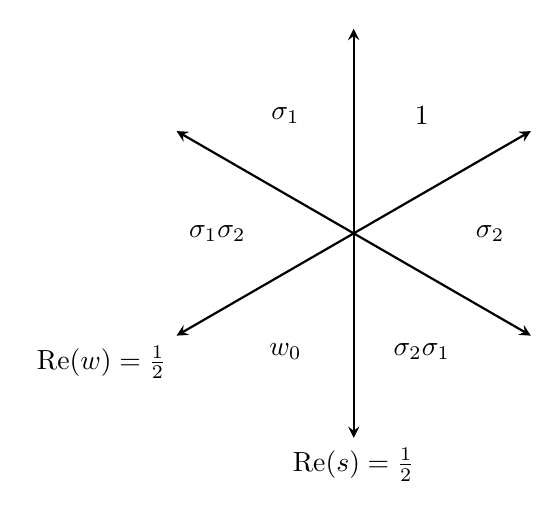
\begin{tikzpicture}[scale=3]
            \draw[thick,-stealth] (0:0) to (30:{sqrt(3)/2});
            \draw[thick,-stealth] (0:0) to (30:{-sqrt(3)/2}) node [below left] {$\Re(w) = \frac{1}{2}$};
            \draw[thick,-stealth] (0:0) to (90:{sqrt(3)/2});
            \draw[thick,-stealth] (0:0) to (90:{-sqrt(3)/2}) node [below] {$\Re(s) = \frac{1}{2}$};
            \draw[thick,-stealth] (0:0) to (150:{sqrt(3)/2});
            \draw[thick,-stealth] (0:0) to (150:{-sqrt(3)/2});

            \node at (60:{sqrt(3)/3}) {$1$};
            \node at (120:{sqrt(3)/3}) {$\s_{1}$};
            \node at (180:{sqrt(3)/3}) {$\s_{1}\s_{2}$};
            \node at (240:{sqrt(3)/3}) {$w_{0}$};
            \node at (300:{sqrt(3)/3}) {$\s_{2}\s_{1}$};
            \node at (0:{sqrt(3)/3}) {$\s_{2}$};
        \end{tikzpicture}
    \end{center}

    In this diagram we have transformed the $(s,w)$-plane so that the origin lies at $\left(\frac{1}{2},\frac{1}{2}\right)$ and the $(s,w)$-axes intersect at $\frac{\pi}{3}$ angles. We have done this so that $\s_{1}$ and $\s_{2}$ act by rigid motions sending the region enclosing $1$ (corresponding to the identity) to either of the adjacent triangles. The other regions are obtained by acting by the corresponding element of $W$. The initial region $\L$ that $Z(s,w)$ is defined on is displayed in the figure below:
    
    \begin{center}
        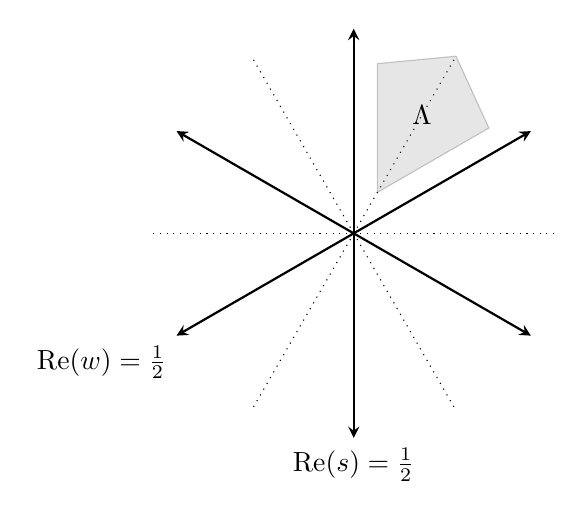
\begin{tikzpicture}[scale=3]
            \draw[dotted](0,0) to (60:{sqrt(3)/2});
            \draw[dotted](0,0) to (240:{sqrt(3)/2});
            \draw[dotted](0,0) to (180:{sqrt(3)/2});
            \draw[dotted](0,0) to (360:{sqrt(3)/2});
            \draw[dotted] (0:0) to (120:{sqrt(3)/2});
            \draw[dotted] (0:0) to (300:{sqrt(3)/2});

            \draw[thick,-stealth] (0:0) to (30:{sqrt(3)/2});
            \draw[thick,-stealth] (0:0) to (30:{-sqrt(3)/2}) node [below left] {$\Re(w) = \frac{1}{2}$};
            \draw[thick,-stealth] (0:0) to (90:{sqrt(3)/2});
            \draw[thick,-stealth] (0:0) to (90:{-sqrt(3)/2}) node [below] {$\Re(s) = \frac{1}{2}$};
            \draw[thick,-stealth] (0:0) to (150:{sqrt(3)/2});
            \draw[thick,-stealth] (0:0) to (150:{-sqrt(3)/2});


            \draw[fill=gray,opacity=0.2] (60:0.2) --+ (0,{((sqrt(5)/3)-0.2)}) -- (60:{sqrt(3)/2}) -- ($(60:0.2)+(30:{((sqrt(5)/3)-0.2)})$) -- cycle;

            \node at (60:{sqrt(3)/3}) {$\L$};
        \end{tikzpicture}
    \end{center}
    
     To meromorphically continue $Z(s,w)$ to all of the $(s,w)$-plane, we first need to show that the quadratic double Dirichlet series $Z_{a_{1},a_{2}}(s,w)$ are locally absolutely uniformly convergent on a slightly larger region than $\L$. This will be achieved by the Phragm\'en-Lindel\"of convexity principal. Fix some small $\e > 0$. The functional equations for $L^{\ast}(s,\chi_{a_{1}d})$ and $L^{\ast}(w,\wtilde{\chi}_{a_{2}m})$ and Stirling's formula together imply the estimates
    \[
        L(-\e,\chi_{a_{1}d}) \ll (a_{1}d)^{\frac{1}{2}+\e} \quad \text{and} \quad L(-\e,\wtilde{\chi}_{a_{2}m}) \ll (a_{2}m)^{\frac{1}{2}+\e},
    \]
    because $L(1+\e,\chi_{a_{1}d}) \ll 1$ and $L(1+\e,\wtilde{\chi}_{a_{2}m}) \ll 1$. As both of these $L$-functions have at most a simple pole at $s = 1$ and $w = 1$ respectively, the Phragm\'en-Lindel\"of convexity principal gives the weak estimates
    \[
        (s-1)L(s,\chi_{a_{1}d}) \ll (a_{1}d)^{\frac{1}{2}+\e} \quad \text{and} \quad (w-1)L(w,\wtilde{\chi}_{a_{2}m}) \ll (a_{2}m)^{\frac{1}{2}+\e},
    \]
    and hence
    \[
        (s-1)L^{(2)}(s,\chi_{a_{1}d}) \ll (a_{1}d)^{\frac{1}{2}+\e} \quad \text{and} \quad (w-1)L^{(2)}(w,\wtilde{\chi}_{a_{2}m}) \ll (a_{2}m)^{\frac{1}{2}+\e},
    \]
    for $\Re(s) > -\e$ and $\Re(w) > -\e$. It follows from the interchange that $(s-1)(w-1)Z_{a_{1},a_{2}}(s,w)$ is locally absolutely uniformly convergent on the region
    \[
        \L_{0} = \L \cup \left\{(s,w) \in \C^{2}:\Re(s) > 0, \Re(w) > \frac{3}{2}\right\} \cup \left\{(s,w) \in \C^{2}:\Re(s) > \frac{3}{2}, \Re(w) > 0\right\}.
    \]
    
    \begin{center}
        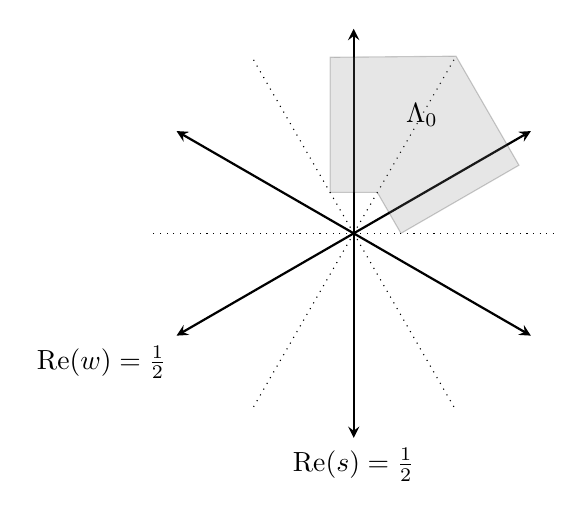
\begin{tikzpicture}[scale=3]
            \draw[dotted](0,0) to (60:{sqrt(3)/2});
            \draw[dotted](0,0) to (240:{sqrt(3)/2});
            \draw[dotted](0,0) to (180:{sqrt(3)/2});
            \draw[dotted](0,0) to (360:{sqrt(3)/2});
            \draw[dotted] (0:0) to (120:{sqrt(3)/2});
            \draw[dotted] (0:0) to (300:{sqrt(3)/2});

            \draw[thick,-stealth] (0:0) to (30:{sqrt(3)/2});
            \draw[thick,-stealth] (0:0) to (30:{-sqrt(3)/2}) node [below left] {$\Re(w) = \frac{1}{2}$};
            \draw[thick,-stealth] (0:0) to (90:{sqrt(3)/2});
            \draw[thick,-stealth] (0:0) to (90:{-sqrt(3)/2}) node [below] {$\Re(s) = \frac{1}{2}$};
            \draw[thick,-stealth] (0:0) to (150:{sqrt(3)/2});
            \draw[thick,-stealth] (0:0) to (150:{-sqrt(3)/2});

            \draw[fill=gray,opacity=0.2] (0:0.2) --+ (30:{cos(30)*((sqrt(3)/2)-0.2)}) -- (60:{sqrt(3)/2}) -- ($(120:0.2)+(0,{sqrt(5)/3-sin(120)*0.2})$) -- (120:0.2) -- (60:0.2) -- cycle;

            \node at (60:{sqrt(3)/3}) {$\L_{0}$};
        \end{tikzpicture}
    \end{center}
    
    Therefore $Z_{a_{1},a_{2}}(s,w)$ is meromorphic on this region with at most polar lines at $s = 1$ and $w = 1$. The key difference between $\L$ and $\L_{0}$ is that $\L_{0}$ intersects the hyperplanes $s = \frac{1}{2}$ and $w = \frac{1}{2}$ so that the union of the reflections $w\L_{0}$ for $w \in W$ is connected. This guarantees that the functional equations imply meromorphic continuation since adjacent reflections of $\L_{0}$ overlap on open sets. We now reflect $\L_{0}$ via the functional equations and then apply a theorem of Bochner which we now state. First, we say that a domain $\W \subset \C^{n}$ is a \textbf{tube domain} if there is an open set $\w \subset \R^{n}$ such that
    \[
        \W = \{(s_{1},\ldots,s_{n}) \in \C^{n}:\Re((s_{1},\ldots,s_{n})) \in \w\}.
    \]
    Tube domains are generalizations of vertical strips in the complex plane. Now we can state the theorem of Bochner (see \cite{hormander2000introduction} for a proof):

    \begin{theorem}[Bochner's continuation theorem]
        If $\W$ is a connected tube domain, then any holomorphic function on $\W$ can be extended to a holomorphic function on the convex hull $\what{\W}$.
    \end{theorem}

    Clearing polar divisors if necessary, Bochner's continuation theorem implies that any meromorphic function on a connected tube domain possessing a finite amount of hyperplane polar divisors can be extended to a meromorphic function on the convex hull. This is exactly the situation for $Z(s,w)$. Clearly $\L_{0}$ is a tube domain and on $\L_{0}$ there are a most polar lines at $s = 1$ and $w = 1$. Reflecting these hyperplanes via $W$ we obtain the finite set of possible polar divisors:
    \[
        \left\{s = 1, w = 1, s = 0, w = 0, s+w = \frac{1}{2}, s+w = \frac{3}{2}\right\}.
    \]
    So by the previous argument, we are reduced to extending $Z(s,w)$ meromorphically. By applying the functional equations corresponding to $\s_{1}$, $\s_{2}$, and $\s_{1}\s_{2}$, $Z(s,w)$ admits meromorphic continuation to the region
    \[
        \L_{12} = \L_{0} \cup \s_{1}\L_{0} \cup \s_{2}\L_{0} \cup \s_{1}\s_{2}\L_{0}.
    \]

    \begin{center}
        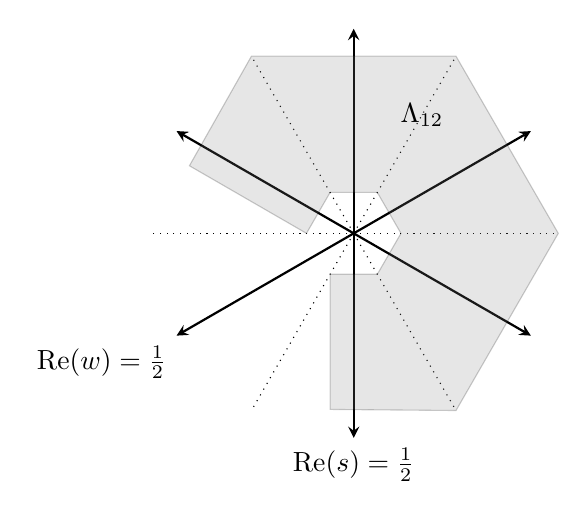
\begin{tikzpicture}[scale=3]
            \draw[dotted](0,0) to (60:{sqrt(3)/2});
            \draw[dotted](0,0) to (240:{sqrt(3)/2});
            \draw[dotted](0,0) to (180:{sqrt(3)/2});
            \draw[dotted](0,0) to (360:{sqrt(3)/2});
            \draw[dotted] (0:0) to (120:{sqrt(3)/2});
            \draw[dotted] (0:0) to (300:{sqrt(3)/2});

            \draw[thick,-stealth] (0:0) to (30:{sqrt(3)/2});
            \draw[thick,-stealth] (0:0) to (30:{-sqrt(3)/2}) node [below left] {$\Re(w) = \frac{1}{2}$};
            \draw[thick,-stealth] (0:0) to (90:{sqrt(3)/2});
            \draw[thick,-stealth] (0:0) to (90:{-sqrt(3)/2}) node [below] {$\Re(s) = \frac{1}{2}$};
            \draw[thick,-stealth] (0:0) to (150:{sqrt(3)/2});
            \draw[thick,-stealth] (0:0) to (150:{-sqrt(3)/2});

            \draw[fill=gray,opacity=0.2] (240:0.2) --+ (0,{-((sqrt(5)/3)+sin(240)*0.2)}) -- (300:{sqrt(3)/2}) -- (0:{sqrt(3)/2}) -- (60:{sqrt(3)/2}) -- (120:{sqrt(3)/2}) -- ($(180:0.2)+(150:{((sqrt(5)/3)+cos(150)*0.2)})$) -- (180:0.2) -- (120:0.2) -- (60:0.2) -- (0:0.2)-- (300:0.2) -- cycle;

            \node at (60:{sqrt(3)/3}) {$\L_{12}$};
        \end{tikzpicture}
    \end{center}

    Now $\L_{12}$ is a connected tube domain whose convex hull is $\C^{2}$. So by applying Bochner's continuation theorem (or rather our comment for meromorphic functions) we see that $Z(s,w)$ admits meromorphic continuation to the $(s,w)$-plane with at most a finite set of polar divisors. This argument is more elegant than repeatedly applying the functional equations corresponding to every $w \in W$. Indeed, if we did we would obtain meromorphic continuation to the region
    \[
        \L_{W} = \bigcup_{w \in W} w\L_{0}.
    \]

    \begin{center}
        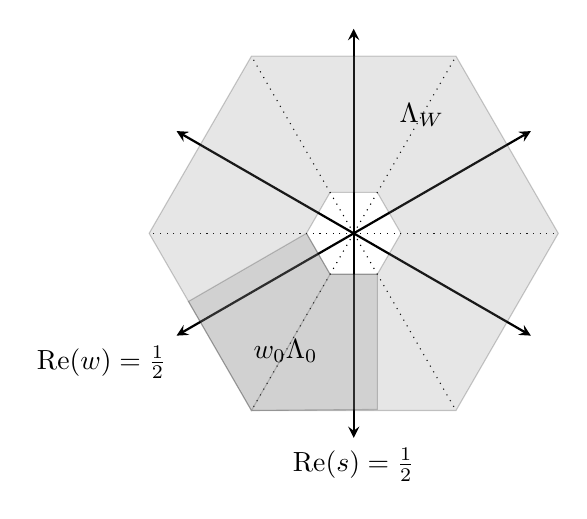
\begin{tikzpicture}[scale=3]
            \draw[dotted](0,0) to (60:{sqrt(3)/2});
            \draw[dotted](0,0) to (240:{sqrt(3)/2});
            \draw[dotted](0,0) to (180:{sqrt(3)/2});
            \draw[dotted](0,0) to (360:{sqrt(3)/2});
            \draw[dotted] (0:0) to (120:{sqrt(3)/2});
            \draw[dotted] (0:0) to (300:{sqrt(3)/2});

            \draw[thick,-stealth] (0:0) to (30:{sqrt(3)/2});
            \draw[thick,-stealth] (0:0) to (30:{-sqrt(3)/2}) node [below left] {$\Re(w) = \frac{1}{2}$};
            \draw[thick,-stealth] (0:0) to (90:{sqrt(3)/2});
            \draw[thick,-stealth] (0:0) to (90:{-sqrt(3)/2}) node [below] {$\Re(s) = \frac{1}{2}$};
            \draw[thick,-stealth] (0:0) to (150:{sqrt(3)/2});
            \draw[thick,-stealth] (0:0) to (150:{-sqrt(3)/2});
        
            \draw[fill=gray,opacity=0.2] (240:{sqrt(3)/2}) -- (300:{sqrt(3)/2}) -- (0:{sqrt(3)/2}) -- (60:{sqrt(3)/2}) -- (120:{sqrt(3)/2}) -- (180:{sqrt(3)/2}) -- (240:{sqrt(3)/2}) -- (240:0.2) -- (180:0.2) -- (120:0.2) -- (60:0.2) -- (0:0.2) -- (300:0.2) -- (240:0.2) -- cycle;

            \draw[fill=gray,opacity=0.2] (180:0.2) --+ (210:{-cos(210)*((sqrt(3)/2)-0.2)}) -- (240:{sqrt(3)/2}) -- ($(300:0.2)+(0,{-((sqrt(5)/3)+sin(300)*0.2)})$) -- (300:0.2) -- (240:0.2) -- cycle; 

            \node at (60:{sqrt(3)/3}) {$\L_{W}$};
            \node at (240:{sqrt(3)/3}) {$w_{0}\L_{0}$};
        \end{tikzpicture}
    \end{center}
    
    There are two issues here. The first is that $Z(s,w)$ has two meromorphic continuations to the region $w_{0}\L_{0}$ given by the functional equations corresponding to $w_{0} = \s_{1}\s_{2}\s_{1}$ and $w_{0} = \s_{2}\s_{1}\s_{2}$ and we would need to show that these agree. The second is that we have not obtained meromorphic continuation to $\C^{2}-\L_{W}$ which is a compact hexagon about the origin. By using Bochner's theorem after meromorphically continuing to $\L_{12}$, we have avoided these issues and as a consequence shown that the meromorphic continuations given by $w_{0} = \s_{1}\s_{2}\s_{1}$ and $w_{0} = \s_{2}\s_{1}\s_{2}$ agree.
\section{Poles \& Residues}
    We can now determine the poles and residues of $Z(s,w)$. Recall that the set of possible polar divisors is
    \[
        \left\{s = 1, w = 1, s = 0, w = 0, s+w = \frac{1}{2}, s+w = \frac{3}{2}\right\}.
    \]
    The poles of $Z(s,w)$ is actually smaller than this set as there are no poles on the hyperplanes $s = 0$, $w = 0$, and $s+w = \frac{3}{2}$. To see this, first observe that by our earlier application of the Phragm\'en-Lindel\"of convexity principal we actually obtained continuation to an open set containing $\L_{0}$ (because our estimates held for $\Re(s) > -\e$ and $\Re(w) > -\e$). We did not need this slightly larger region for the meromorphic continuation but we do require it to study the poles. Now consider the possible polar divisor $s = 0$. Therefore $(s-1)(w-1)Z_{a_{1},a_{2}}(s,w)$ is holomorphic on an open set containing $\L_{0}$ which contains half of the hyperplane defined by $s = 0$ outside of the hexagon $\C^{2}-\L_{W}$. Since $(s-1)(w-1)$ is holomorphic on this region, $Z_{a_{1},a_{2}}(s,w)$ can not have a polar divisor at $s = 0$ on an open set containing $\L_{0}$. Moreover, an open set containing $\s_{1}\s_{2}\L_{0}$ contains the other half of the hyperplane defined by $s = 0$ outside of the hexagon $\C^{2}-\L_{W}$. Upon applying the functional equation corresponding to $\s_{1}\s_{2}$, \cref{thm:double_Dirichlet_series_functional_equation} implies that the gamma factors in the corresponding functional equation have a simple pole when $s+w = \frac{3}{2}$ (the gamma factors in the functional equation for $\s_{1}$ have a simple pole at $s = 1$ and $s-1 \to s+w-\frac{3}{2}$ under $\s_{2}$). Therefore $Z_{a_{1},a_{2}}(s,w)$ does not have polar divisors at $s = 0$ on an open set containing $\s_{1}\s_{2}\L_{0}$ away from $s+w = \frac{3}{2}$. In particular, $Z(s,w)$ does not have a polar divisor at $s = 0$ on $\L_{W}$ and away from the other polar divisors. By Bochner's continuation theorem (after clearing all of the other possible polar divisors), $Z(s,w)$ does not have a polar divisors at $s = 0$ on all of $\C^{2}$ and away from the other polar divisors. An identical argument holds for the case $w = 0$ using the regions $\L_{0}$ and $\s_{2}\s_{1}\L_{0}$. For the polar divisor $s+w = \frac{1}{2}$, we argue in the same way with the regions $\s_{2}\s_{1}\L_{0}$, $\s_{1}\s_{2}\L_{0}$, and $w_{0}\L_{0}$, but there is one difference. For these regions, the gamma factors in the corresponding functional equations are different. For the first two regions $\s_{2}\s_{1}\L_{0}$ and $\s_{1}\s_{2}\L_{0}$, the gamma factors have a simple pole when $s+w = \frac{3}{2}$. For the third region $w_{0}\L_{0}$, the gamma factors have simple poles at $s = 1$ and $w = 1$ which is seen by using both representations $w_{0} = \s_{1}\s_{2}\s_{1}$ and $w_{0} = \s_{2}\s_{1}\s_{2}$. Nevertheless, there are no poles on the hyperplanes $s = 0$, $w = 0$, and $s+w = \frac{1}{2}$ and away from the other polar divisors. As for the hyperplanes $s = 1$, $w = 1$, and $s+w = \frac{3}{2}$, there are clearly genuine poles for $s = 1$ and $w = 1$ coming from $L(s,\chi_{d_{0}})$ and $L(w,\chi_{m_{0}})$ when $d$ and $m$ are perfect squares (so that $d_{0} = m_{0} = 1$). For $s+w = \frac{3}{2}$, we have a pole coming from the gamma factors corresponding to the functional equations for $\s_{2}\s_{1}$ and $\s_{1}\s_{2}$. We collect all of our work as a theorem:

    \begin{theorem}
        $Z(s,w)$ admits meromorphic continuation to $\C^{2}$ with polar divisors $s = 1$, $w = 1$, and $s+w = \frac{3}{2}$.
    \end{theorem}

    We can also study the residues of $Z(s,w)$ at these poles. Since all of the poles are obtained from each other by applying the functional equations of $Z(s,w)$, we begin by looking at the pole when $w = 1$. To compute the residue we use the representation
    \[
        Z(s,w) = \sum_{\substack{m \ge 1 \\ (m,2) = 1}}\frac{L^{(2)}(w,\wtilde{\chi}_{m_{0}})Q_{m_{0}m_{1}^{2}}(w)}{m^{s}},
    \]
    coming from the interchange. The numerator $L(w,\wtilde{\chi}_{m_{0}})Q_{m_{0}m_{1}^{2}}(w)$ in the summand corresponding to $m$ has a pole at $w = 1$ if and only if $m_{0}$ is a perfect square, that is $m_{0} = 1$, or equivalently $m = m_{1}^{2}$ itself is a perfect square. In this case, $L(w,\wtilde{\chi}_{m_{0}}) = \z(w)$ and
    \[
        \Res_{w = 1}L^{(2)}(w,\chi_{m_{0}})Q_{m_{0}m_{1}^{2}}(w) = \frac{1}{2}Q_{m_{1}^{2}}(1).
    \]
    But from \cref{lem:prime_correction_even,thm:correction_polynomial_Euler_product} we see that $Q_{m_{1}^{2}}(1) = 1$, and hence
    \[
        \Res_{w = 1}Z(s,w) = \frac{1}{2}\sum_{\substack{\text{$m$ perfect square} \\ (m,2) = 1}}\frac{Q_{m_{1}^{2}}(1)}{m^{s}} = \frac{1}{2}\sum_{\substack{m \ge 1 \\ (m,2) = 1}}\frac{1}{m^{2s}} = \frac{1}{2}\z^{(2)}(2s).
    \]
    Notice that this expression has a simple pole at $s = \frac{1}{2}$ which is exactly when the polar lines $w = 1$ and $s+w = \frac{3}{2}$ intersect. The residue of $Z(s,w)$ at $s = 1$ is computed in an analogous way. Indeed, by applying the interchange, the exact same argument holds with the roles of $s$ and $w$ interchanged so that
    \[
        \Res_{s = 1}Z(s,w) = \frac{1}{2}\z^{(2)}(2w).
    \]
    Again, this expression has a simple pole at $w = \frac{1}{2}$ which is when the polar lines $s = 1$ and $s+w = \frac{3}{2}$ intersect. The other residues at the simple poles can be computed by applying the functional equations for $Z(s,w)$ and using the residues at $s = 1$ and $w = 1$. Now consider the point where the polar lines $w = 1$ and $s+w = \frac{3}{2}$ intersect. Setting $s = \frac{1}{2}$, we see that $Z\left(\frac{1}{2},w\right)$ has a pole at $w= 1$ and we would like to study this pole more. To achieve this, the Mittag-Leffler theorem applied to $Z(s,w)$ (in $w$) implies
    \[
        Z(s,w) = \frac{R_{1}(s)}{w-1}+\frac{R_{2}(s)}{s+w-\frac{3}{2}}+V(s,w),
    \]
    in some neighborhood of $\left(\frac{1}{2},1\right)$, where $V(s,w)$ is holomorphic, and we have set
    \[
        R_{1}(s) = \Res_{w = 1}Z(s,w) \quad \text{and} \quad R_{2}(s) = \Res_{w = \frac{3}{2}-s}Z(s,w).
    \]
    From our residue computations above, $R_{1}(s) = \frac{1}{2}\z^{(2)}(2s)$ which implies that it has a simple pole at $s = \frac{1}{2}$. The residue is given by $A = \frac{1}{8}$. On the other hand, $Z\left(\frac{1}{2},w\right)$ is holomorphic for $\Re(w) > 1$. These two facts together imply that $R_{2}(s)$ must have a simple pole at $s = \frac{1}{2}$ which cancels the simple pole coming from $R_{1}(s)$. So by Mittag-Leffler again, we may write
    \[
        R_{1}(s) = \frac{A}{s-\frac{1}{2}}+R_{3}(s) \quad \text{and} \quad R_{2}(s) = -\frac{A}{s-\frac{1}{2}}+R_{4}(s),
    \]
    in a neighborhood of $s = \frac{1}{2}$ and where $R_{3}(s)$ and $R_{4}(s)$ are holomorphic. Then
    \begin{align*}
        Z(s,w) &= \frac{R_{1}(s)}{w-1}+\frac{R_{2}(s)}{s+w-\frac{3}{2}}+V(s,w) \\ 
        &= \frac{A}{(w-1)\left(s-\frac{1}{2}\right)}+\frac{R_{3}(s)}{w-1}-\frac{A}{\left(s+w-\frac{3}{2}\right)\left(s-\frac{1}{2}\right)}+\frac{R_{4}(s)}{s+w-\frac{3}{2}}+V(s,w) \\
        &= \frac{A}{(w-1)\left(s+w-\frac{3}{2}\right)}+\frac{R_{3}(s)}{w-1}+\frac{R_{4}(s)}{s+w-\frac{3}{2}}+V(s,w).
    \end{align*}
    We can now set $s = \frac{1}{2}$ and let $B = R_{3}\left(\frac{1}{2}\right)+R_{4}\left(\frac{1}{2}\right)$ so that
    \[
        Z\left(\frac{1}{2},w\right) = \frac{A}{(w-1)^{2}}+\frac{B}{w-1}+O(1).
    \]
    It follows that $Z\left(\frac{1}{2},w\right)$ has a double pole at $w = 1$. This can be thought of as follows: the polar lines $w = 1$ and $s+w = \frac{3}{2}$ correspond to simple poles of $Z(s,w)$ except in the case when they intersect and the order of the poles combine to give $Z\left(\frac{1}{2},w\right)$ a double pole at $w = 1$. Applying the interchange, the exact same argument holds to show that $Z\left(s,\frac{1}{2}\right)$ has a double pole at $s = 1$. We collect this work as a theorem:

    \begin{theorem}\label{thm:double_poles_at_1/2}
        $Z\left(\frac{1}{2},w\right)$ and $Z\left(s,\frac{1}{2}\right)$ have double poles at $w = 1$ and $s = 1$ respectively. In particular, in neighborhoods of $w = 1$ and $s = 1$ respectively, we have
        \[
            Z\left(\frac{1}{2},w\right) = \frac{A}{(w-1)^{2}}+\frac{B}{w-1}+O(1) \quad \text{and} \quad Z\left(s,\frac{1}{2}\right) = \frac{A}{(s-1)^{2}}+\frac{B}{s-1}+O(1),
        \]
        for some constants $A$ and $B$ with $A = \frac{1}{8}$. 
    \end{theorem}

    \bibliographystyle{plain}
    \bibliography{Twiss2024quadratic(II)}

\end{document}